\clearpage

\graphicspath{{./figures/}}
\section{Net2Plan Guide}\label{net2plan_guide}
This first section will describe how to install Net2Plan and some of the solvers.


    \subsection*{Net2Plan Download and Installation}
    \vspace{0.5cm}

    In the software folder (NetPlanner/software/net2plan) there is a stable version of all required installers or programs.

	Before downloading Net2Plan, the first step is verifying if the computer has the necessary Java Runtime Environment.
    The Java Runtime Environment is necessary as Net2Plan was coded in Java.
    Version 8 or later is recommended.
    In the software folder you can find an installer for the Java SE Runtime Environment 8 Update 151, file JavaSetup8u151.exe.
    The latest available version can be found in the Java website at \url{https://java.com/en/download/}.
		
    Having installed the Java Environment it is now possible to run Net2Plan.
    It is possible to run Net2Plan (version  0.4.2) directly from the folder NetPlanner/software/net2plan-0.4.2.
    There is also available a zip file from which the program can be extracted.
    The program can be started just double clicking on the file Net2Plan.jar.
    The latest available version can be found in the Net2Plan website at \url{http://net2plan.com/download.php}.

    \begin{figure}[h!]
       	\centering
       	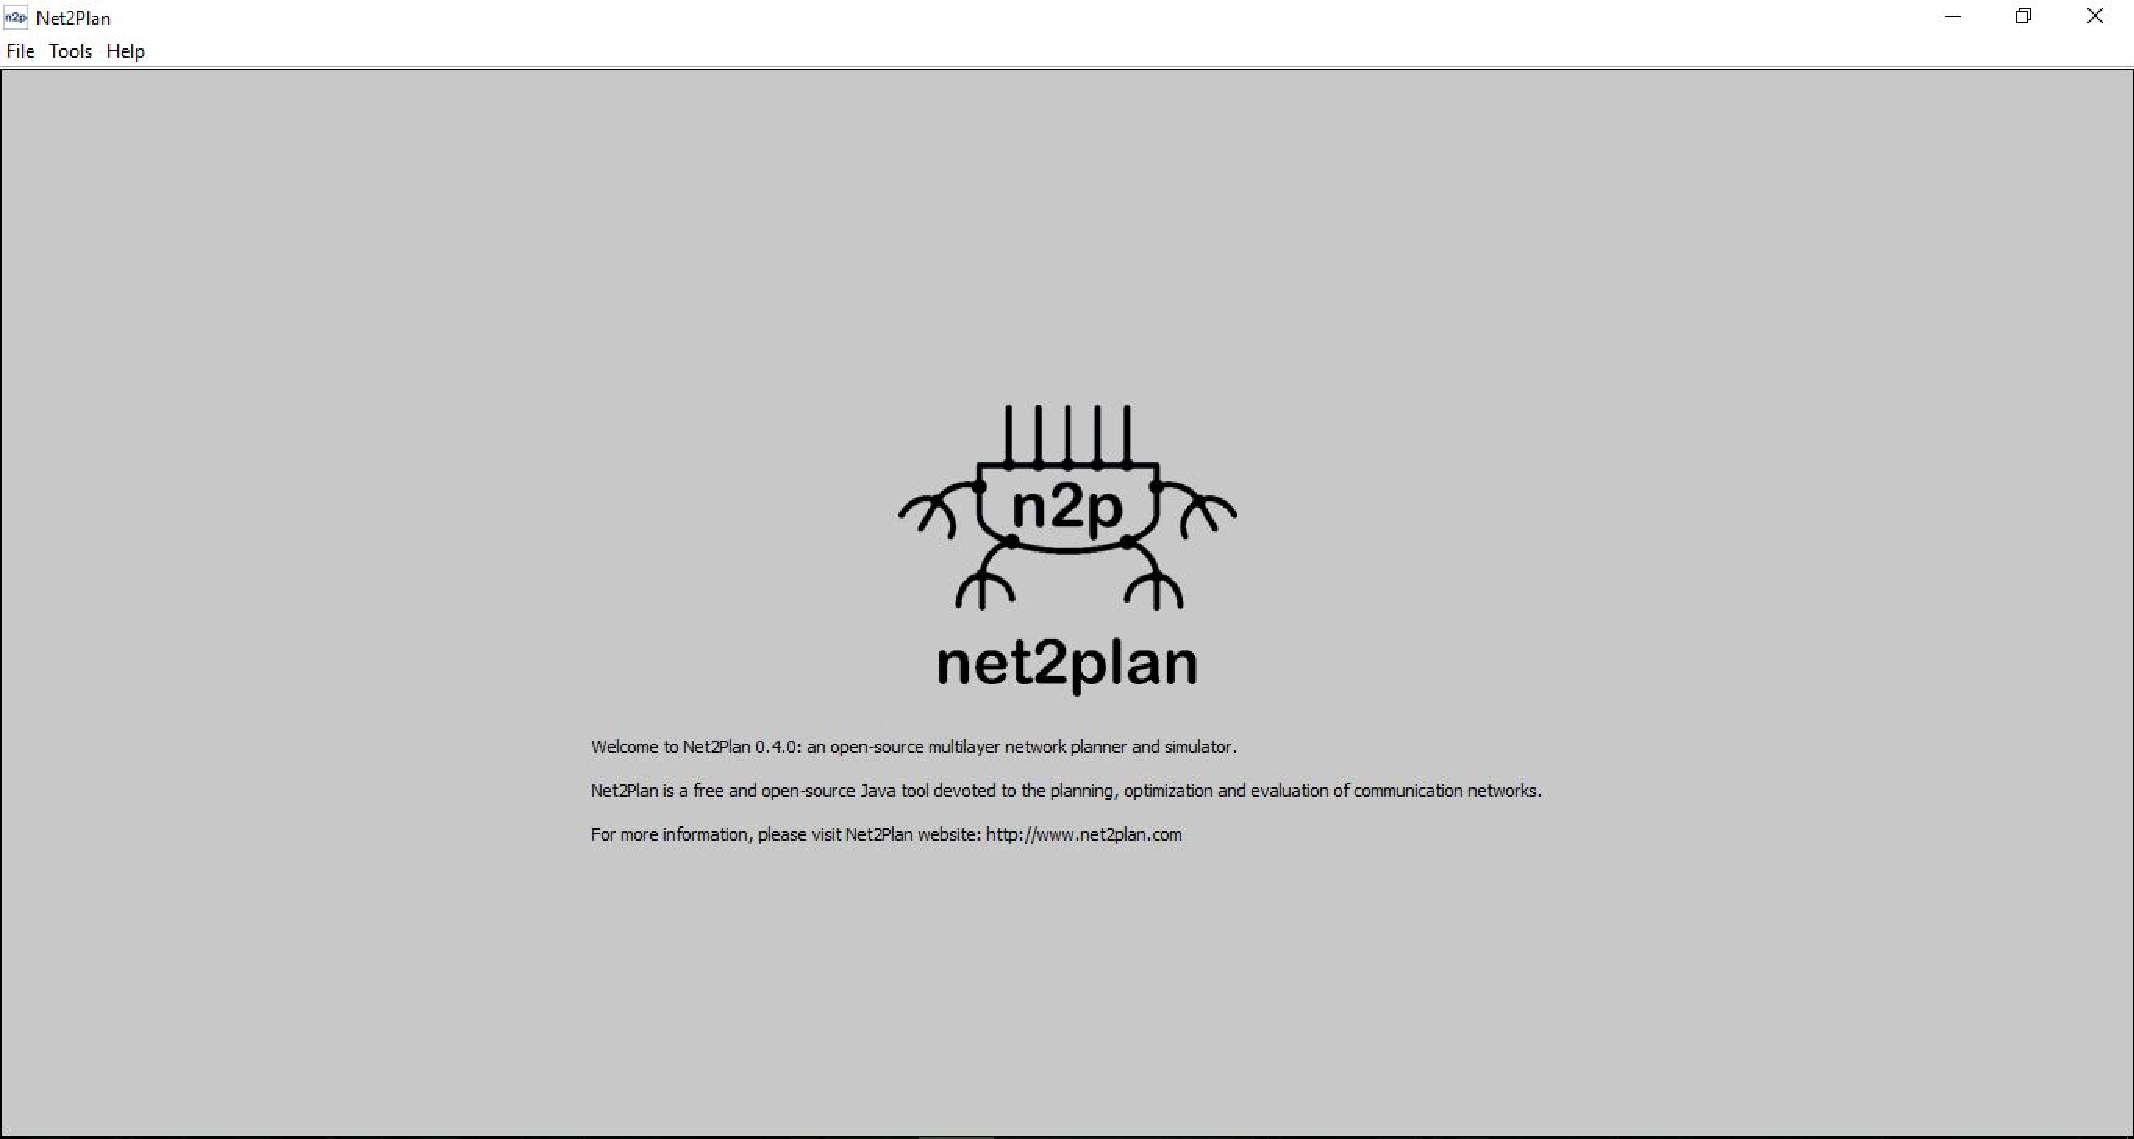
\includegraphics[width = 13cm]{Net2Plan.pdf}
       	\caption{Net2Plan v0.4.2. opening menu.}
    \end{figure}

	\subsection*{Net2Plan Options and Installing Solvers}
	\vspace{0.5cm}
	To access the main Net2Plan options click "File $\rightarrow$ Options". In this window the global parameters for simulations can be changed if needed.
	For example, an important option to note in this tab is the parameter "defaultRunnableCodePath", whose value should be the path to the jar file containing NetPlanner algorithms. As will be explained further on, Net2Plan is an open source tool and as such, new algorithms can be implemented and the default path can be changed to the path where those will be available instead of loading them manually each time Net2Plan is opened.	The remaining parameters are related to solver options, which are the default external solvers used and also the path in which the $".dll"$, $".so"$, $".dylib"$ files of each solver are available. By default there is no path for each solver but in this case it was already changed to where the solvers were installed.
	
	\begin{figure} [h!]
		\centering
		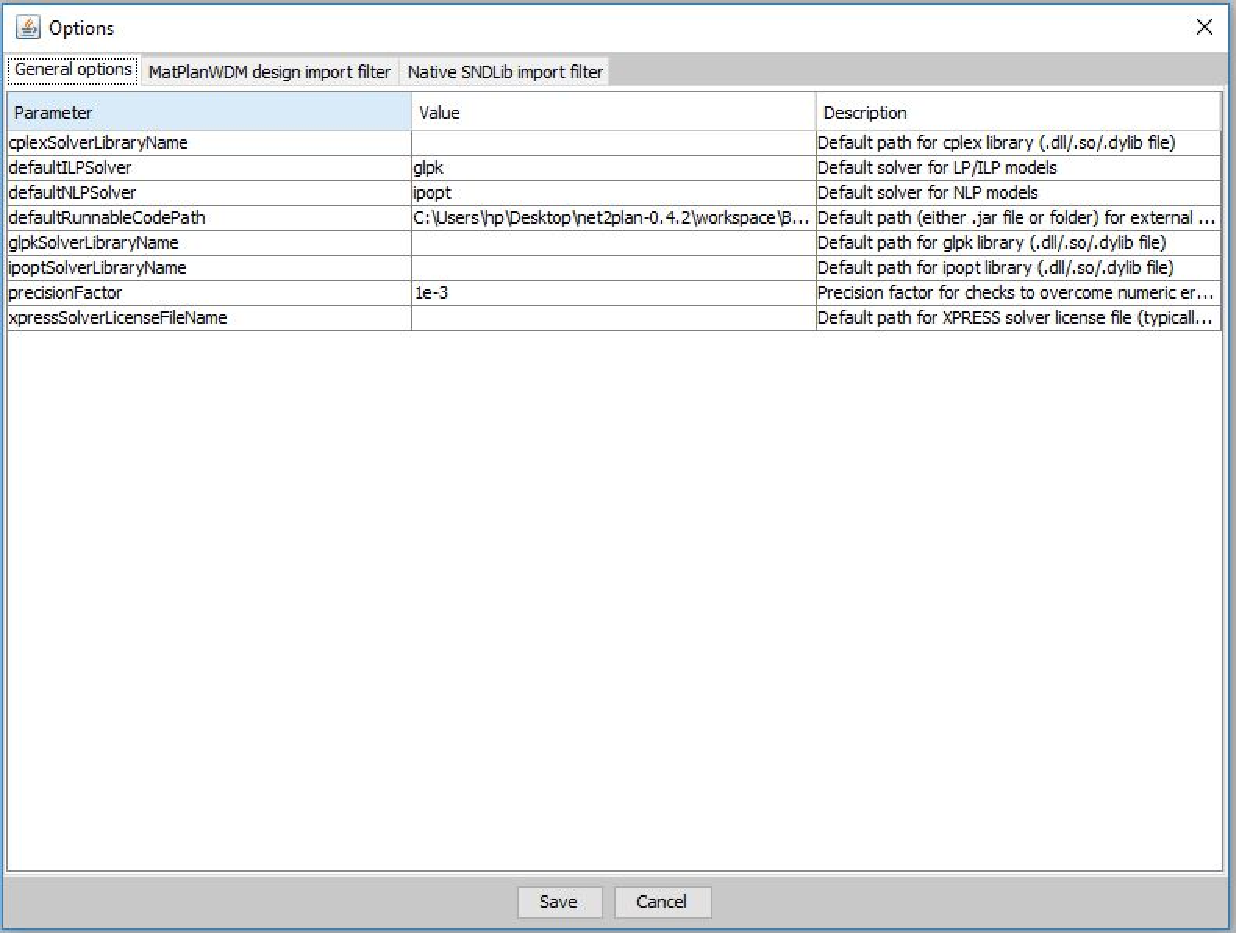
\includegraphics[width = 10cm]{Net2Plan_options.pdf}
		\caption{Net2Plan v0.4.2. general options.}
	\end{figure}
		
	These external solvers are not extracted along with Net2Plan and as such, need to be downloaded if needed for the algorithms to be used.

%As "cplex" is a paid application, only the other two solvers will be shown as the process is similar.\\
%		
%	The "IPOPT" solver can be downloaded from \url{http://www.coin-or.org/download/source/Ipopt/}. There are various choices available to download but for this case the $.dll$ is the main file needed. An example of an algorithm which uses this solver is shown on Figure \ref{Net2Plan_ipopt}. Note that the "solverLibraryName" has the path shown earlier on the "Solver options" tab, this would have to be added manually if not introduced into the main options.
%	
%	\begin{figure}[h!]
%		\centering
%		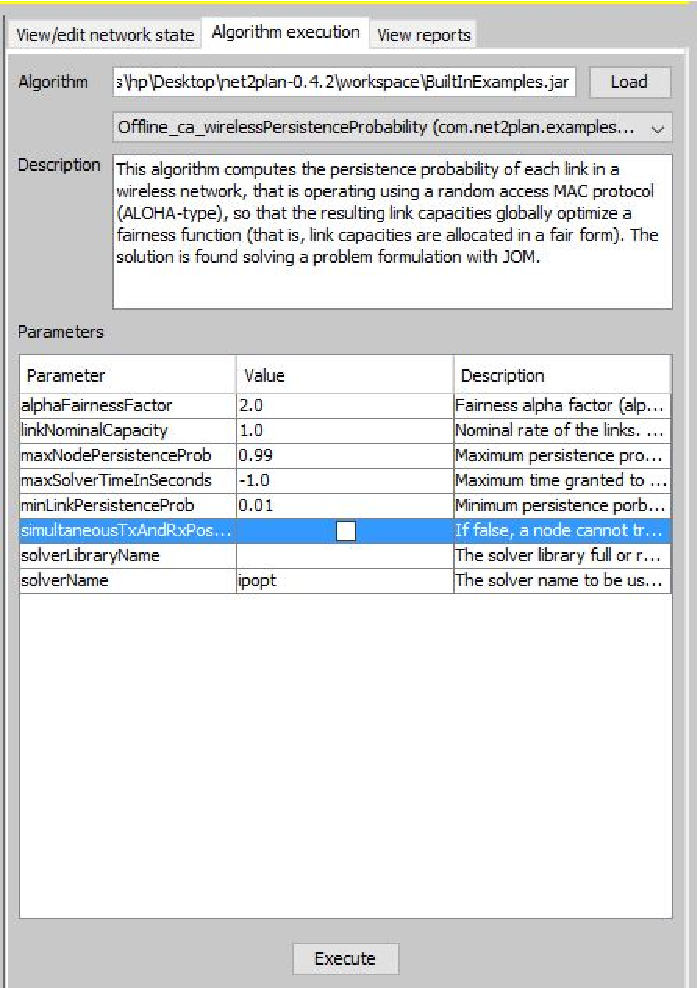
\includegraphics[width = 7cm]{Net2Plan_ipopt.pdf}
%		\caption{Net2Plan Algorithm with $ipopt$ solver}
%		\label{Net2Plan_ipopt}
%	\end{figure}
%		
%	The other free solver also used by some Net2Plan is "glpk", this one can be downloaded from \url{http://sourceforge.net/projects/winglpk/?source=typ_redirect}. An example is shown on Figure \ref{Net2Plan_glpk}. Again note the path shows up as in the options.
%		
%
%	\begin{figure}[h!]
%		\centering
%		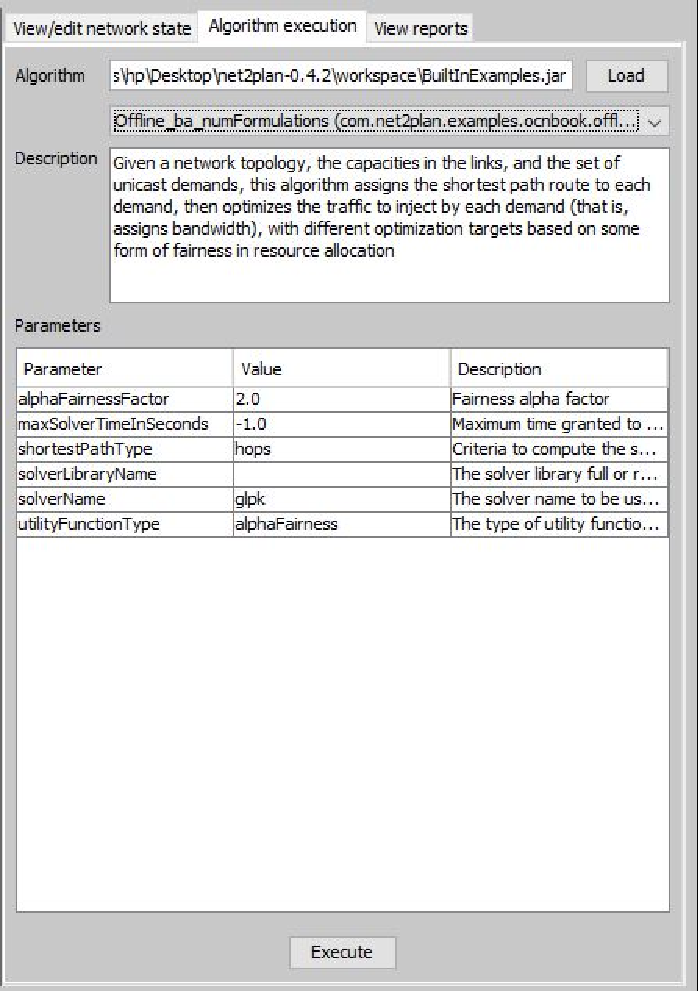
\includegraphics[width = 7cm]{Net2Plan_glpk.pdf}
%		\caption{Net2Plan Algorithm with $glpk$ solver}
%		\label{Net2Plan_glpk}
%	\end{figure}		
%		   	
%    \newpage

\section*{Net2Plan Tools}
This section will describe in some detail the tools presented in Net2Plan as a network planner, most notably how to created a traffic matrix, design a network and some of the simulation options available.

	\subsection*{Creating Traffic Matrices}
    To start creating a traffic matrix in Net2Plan go to "Tools $\rightarrow$ Traffic matrix design" or press $Alt+2$. The traffic matrix menu is shown on Figure \ref{Net2Plan_traffic}.
	
	\begin{figure}[h!]
		\vspace{-0.3cm}
		\centering	
		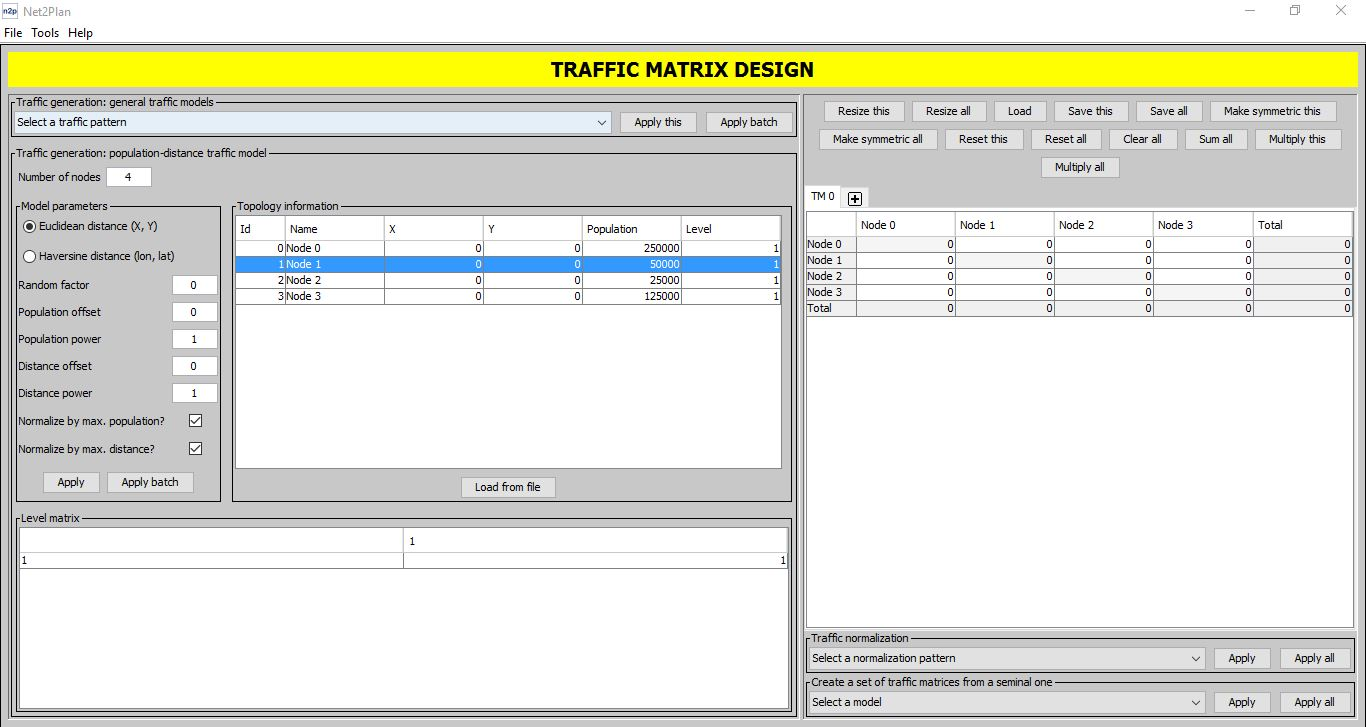
\includegraphics[width = 16cm]{Net2Plan_traffic.pdf}
		\caption{Net2Plan Traffic Matrix Design}
		\label{Net2Plan_traffic}
	\end{figure}
		
	On the top left side a traffic pattern can be chosen for one matrix or several if used the "Apply batch" option.
	
	\begin{itemize}	
		
		\item{"Constant" has two parameters the number of nodes and a constant value. This creates an uniform matrix with the number of nodes chosen and traffic equal to the value selected.}
	
		\item{"Uniform (0,10)" \, has the number of nodes and the option of being symmetric as the parameters. The matrix then has the number of nodes introduced and an amount of traffic chosen randomly between 0 and 10 which can be symmetric or not depending on the choice done.}
	
		\item{"Uniform (0,100)" \, is very similar to the other uniform option whereas in this case the traffic values are chosen randomly between 0 and 100.}
	
		\item{"50\% Uniform (0,100) \& 50\% Uniform (0,10)" \, and "25\% Uniform (0,100) \& 75\% Uniform (0,10)" \, are as expected a mixture of the previous two options.}
	
		\item{"Gravity model" \, in this option a number of nodes is chosen as well as the amount of traffic both generated and received by each node. The sum of the traffic generated by all the nodes needs to be equal to the sum of the traffic received by them. }

	\end{itemize}
	
	Below the traffic pattern options, an existing model can be loaded and additional parameters defined such as Population and Node Level.
	
	On the right side a traffic matrix can be created manually by defining the number of nodes on "resize this" \, and the amount of traffic can be typed on each demand. The other options above the matrix are self explanatory, for example, "multiply this" multiplies all the traffic by a constant number chosen. A point to note is that most options has an "all" choice as it is possible to have more then one matrix created.
	
	Below the matrix part are two further options available for the matrices, the first one is the option to select a normalization pattern such as "Total normalization" where a total number of traffic can be chosen for the network and the demands are adapted to it accordingly. The other option is to create a set of matrices based on the designed one.\\
	
	Figure \ref{TrafficMatrixCreation} shows how to create batch of matrices with constant traffic.
	
	\begin{figure}[h!]
		\centering
		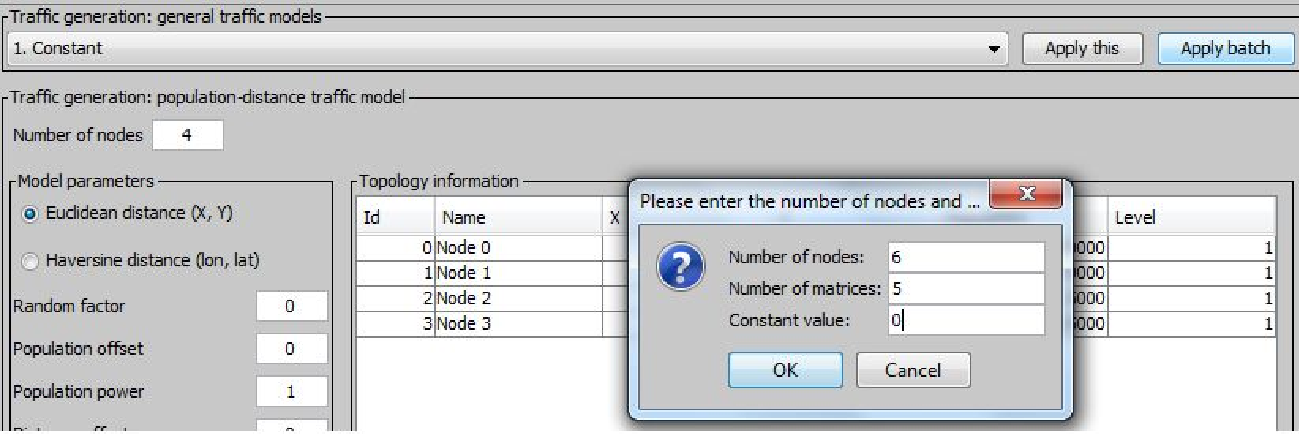
\includegraphics[width = 13cm]{TrafficMatrixCreation.pdf}
		\caption{Net2Plan example on creating a batch of matrices }
		\label{TrafficMatrixCreation}
	\end{figure} 	
	
	Using this option, 5 traffic matrices for a 6 node network were created all with a constant value of 1 as can be seen on figure \ref{Net2Plan_matrix} that shows the first matrix of the batch.

	\begin{figure}[h!]
		\centering
		\includegraphics[width = 13cm]{Net2Plan_matrix.pdf}
		\caption{Net2Plan Traffic Matrix Example}
		\label{Net2Plan_matrix}
	\end{figure}
	
	This example demonstrates how several different types of traffic can be introduced for a network by creating different matrices for each. These can then be saved individually and will further on be used as traffic matrices for ODU's 0 through 4.
	
		
	\subsection*{Creating the Network topologies} \label{Creating the Network topologies}
	To start with the Network creation tools in Net2Plan go to "Tools $\rightarrow$ Offline network design" or press $Alt+1$. The network design menu is shown on Figure \ref{Net2Plan_Network}.
	
	\begin{figure}[h!]
		\centering
		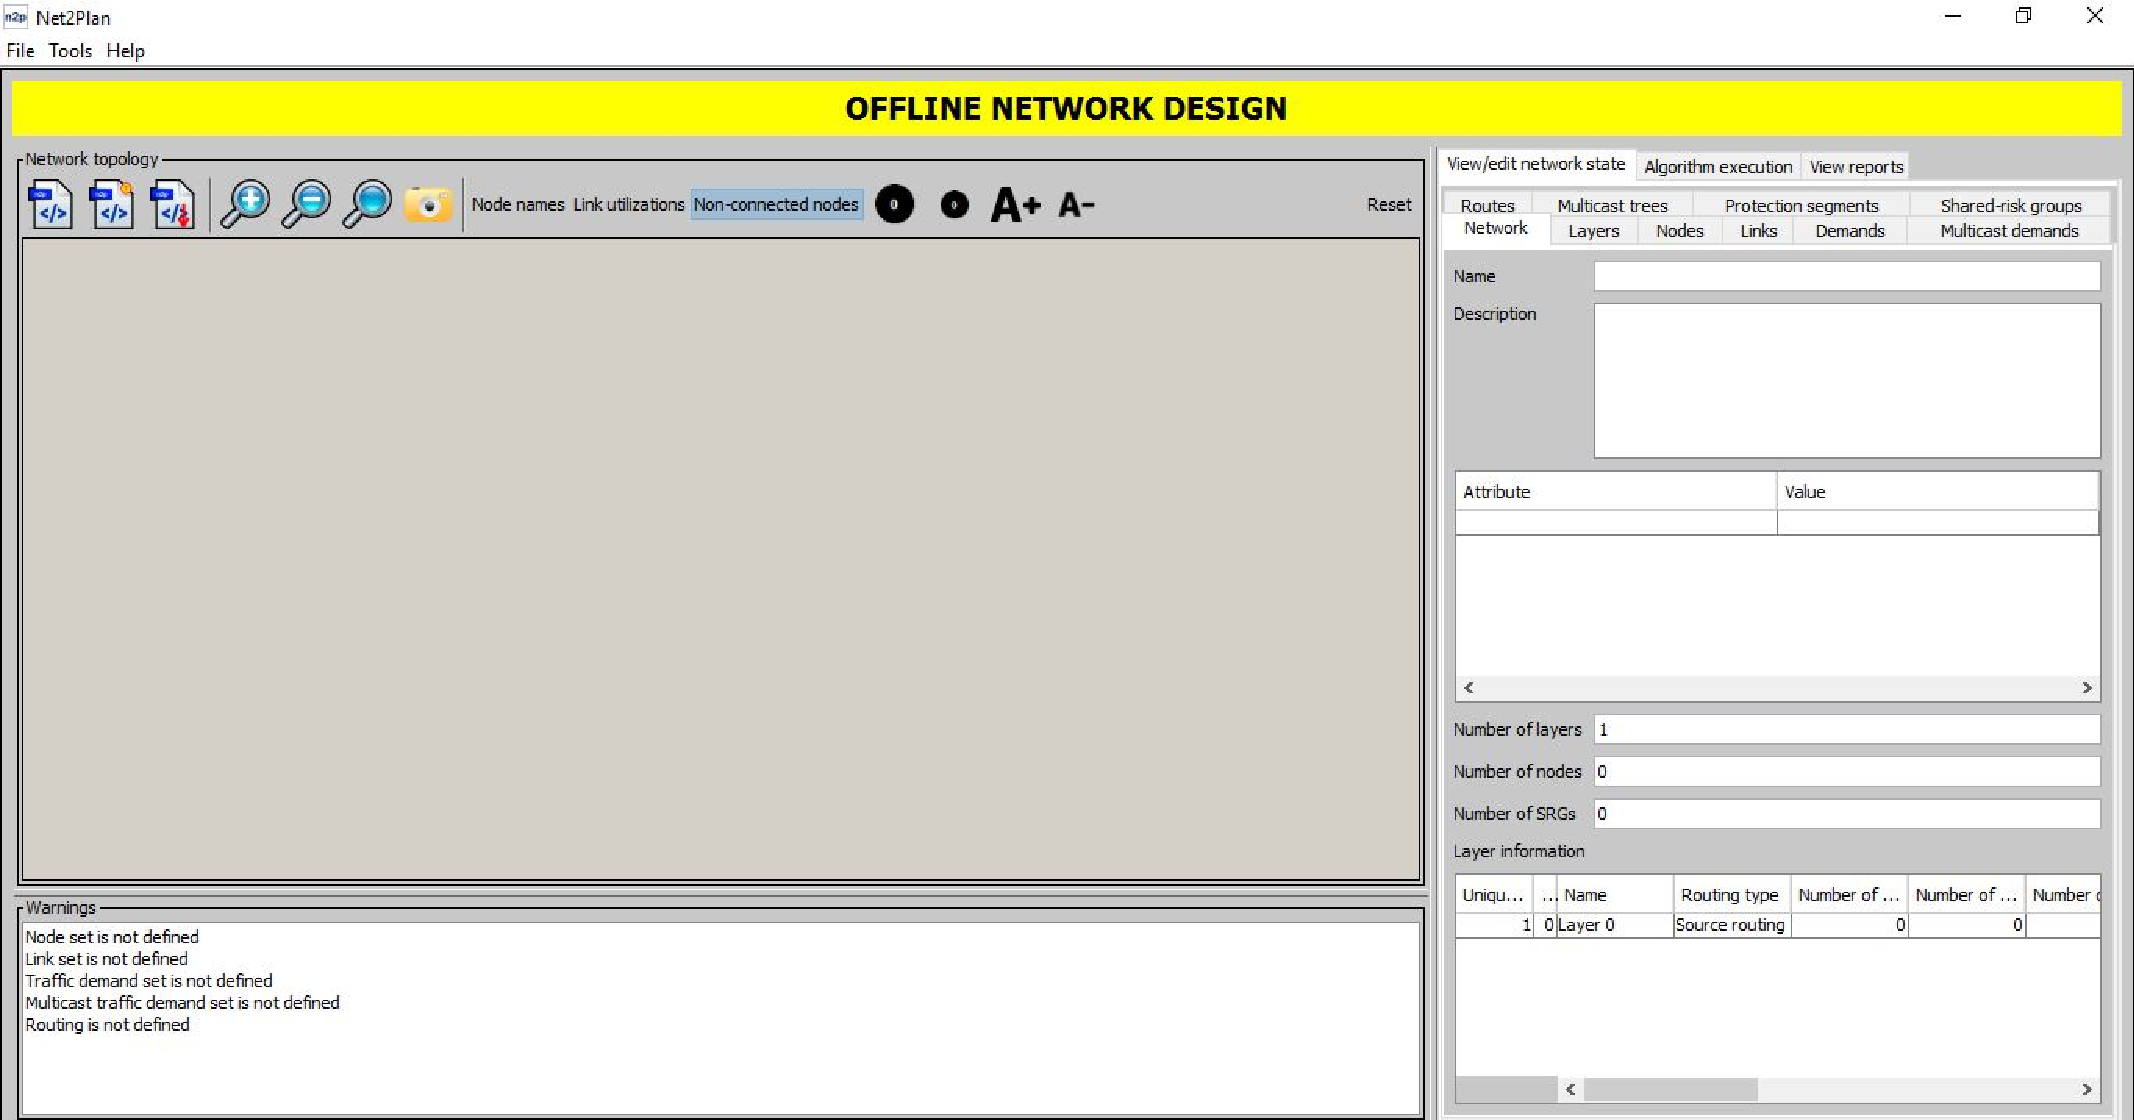
\includegraphics[width = 17cm]{Net2Plan_Network.pdf}
		\caption{Net2Plan Offline Network Design}
		\label{Net2Plan_Network}
	\end{figure}
	
	On the left side, the network topology part has the option to load an existing design and demand set or a new one can be created. To start creating a new network, first nodes have to be introduced by right clicking on the grey area and choosing "Add node here". Links between nodes are created by holding a click on the origin node and dragging until the destination node, holding shift before releasing the click creates 2 links, one in each direction. Another option to create links is to right click on an existing node and choosing the desired create a link option. Nodes can be moved by holding control and dragging them into the desired position.\\
	
	Below the network topology is the "Warnings" box where the parts missing from having a functional network are displayed. For example if the nodes and links where already created it should say "traffic demand set is not defined" and "Routing is not defined" as these were still not introduced.\\
	
	The whole right side of the network design menu are the parameters separated into various tabs which will be explored further on in this document. Besides these tabs, there is also the tab for Algorithm execution where the network is modified based on built algorithms, for example a routing algorithm and the View reports tab where information on the network can be displayed from built in reports. \\

	Figure \ref{Net2Plan_Network_1} demonstrates an example of the 6 node and 16 links network created using the tools explained above. As can be seen on the image at the warning tab, this network sill has several steps left to become a fully functional network. The link capacity will be defined based on the routing algorithm chosen and the demand set will be loaded based on the matrices created. \\
		
	\pagebreak
	\begin{figure}[h!]
		\centering
		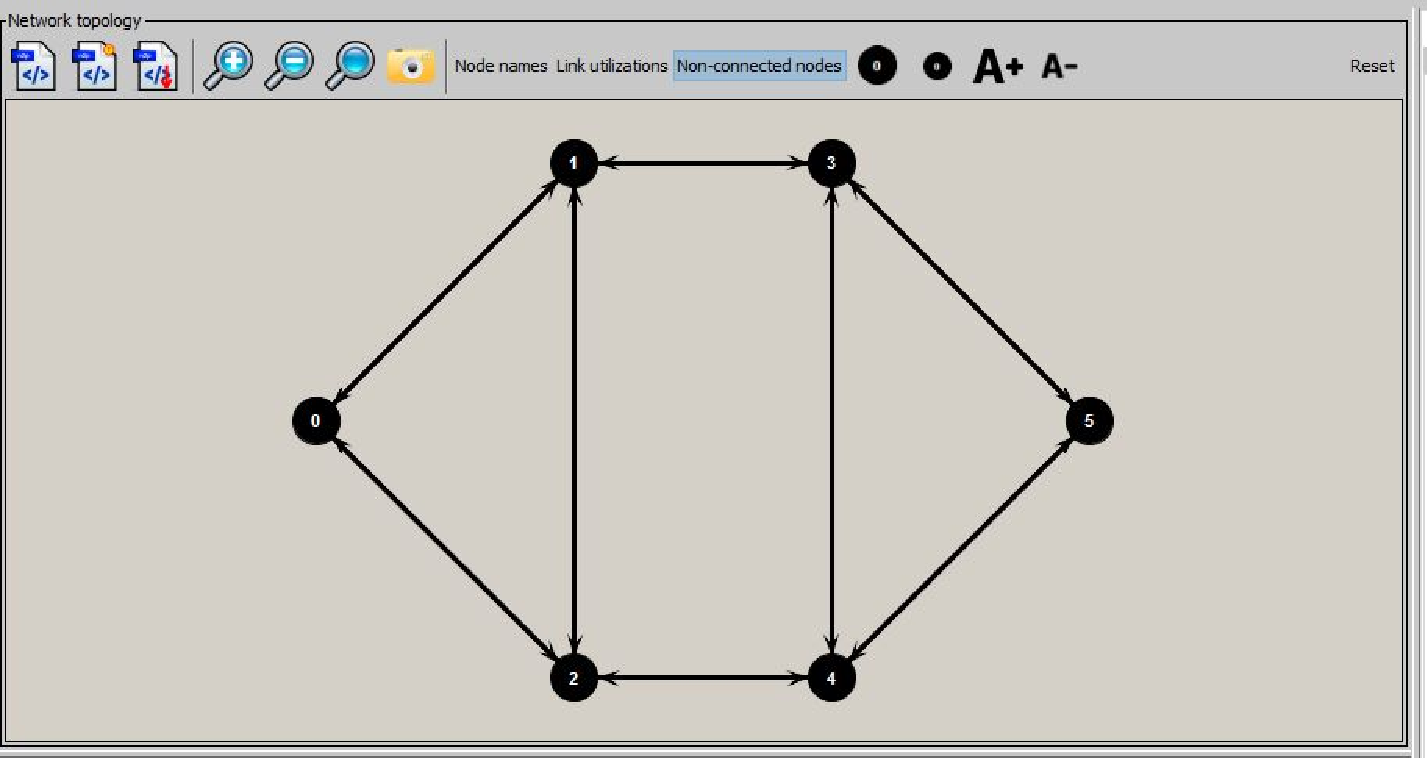
\includegraphics[width = 12cm]{Net2Plan_Network_1.pdf}
		\caption{Net2Plan Network Example}
		\label{Net2Plan_Network_1}
	\end{figure}

	The links and nodes parameters created for the network can be visualized and modified as seen on Figures \ref{Net2Plan_Network_Parameters_a} and \ref{Net2Plan_Network_Parameters_b} displaying the tabs for each case.
	

	\begin{figure}[!h]
		\centering
		\subfigure[a]
		{
			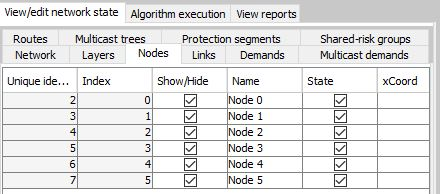
\includegraphics[width=8cm]{Net2Plan_Network_Parameters.pdf}
			\label{Net2Plan_Network_Parameters_a}
		}
		\subfigure[b]
		{
			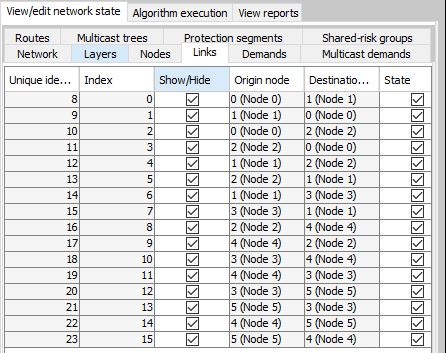
\includegraphics[width=8cm]{Net2Plan_Network_Parameters_1.pdf}
			\label{Net2Plan_Network_Parameters_b}
		}
		\caption{Network a) Nodes tab ; b) Links tab}
	\end{figure}	
	
	On the Nodes tab most of the parameters are still 0 as there is no traffic on the network but there are three parameters that can be changed here. A node name can be set and both x and y coordinates can be defined as a more thorough alternative to define the node position.
	
	On the links tab, again most is at 0 at this moment while the parameters that can be manually set are the link capacity, at 0 until defined and the link length which was set to the same value in every link.\\
	
	Having the basic physical topology created, the next step is to load the demand set into the network. In the case where there are multiple traffic matrices an algorithm was developed to aggregate these in order for it to be possible to load all demands.
	For traffic matrices with ODU signals, an algorithm called "joinTrafficMatrices" can aggregate the different ODUs and convert them to ODU0 in order to have all the traffic in the same units. Besides converting the different ones to ODU0 it also creates an attribute in each demand indicating the type of signal before converting. This attribute can be seen on the demands tab after loading the resulting demand list. Figure \ref{joinMatrices} shows the algorithm to be used.
	

	\begin{figure}[h!]
		\centering
		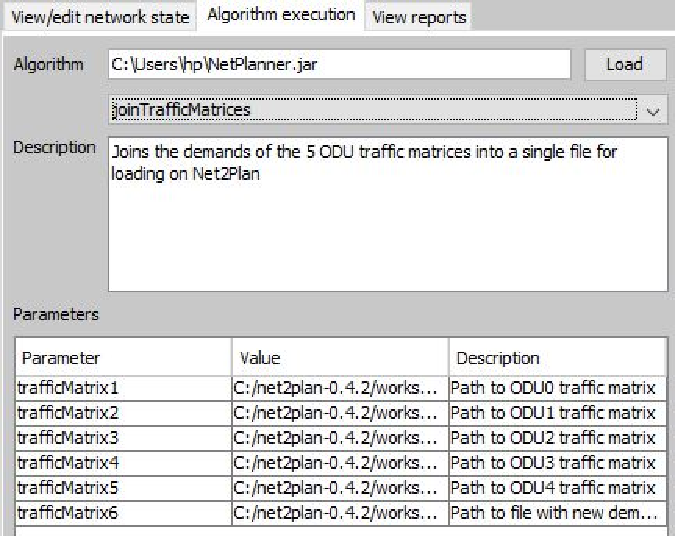
\includegraphics[width=11cm]{Net2Plan_joinMatrices.pdf}
		\caption{joinTrafficMatrices Algorithm}
		\label{joinMatrices}		
	\end{figure}
	
	As can be seen on Figure \ref{joinMatrices} there are 6 user defined parameters, the first five are the paths for the traffic matrices to be aggregated in order, as said in the description. The last parameter is the resulting demand list that can then be loaded into the network.
	
	The paths are by default defined considering Net2Plan is on C:\ and the matrices are in the default directory were they are saved. Lastly, the name of the files are in order ODU0.n2p through ODU4.n2p. All the path and file names can be changed to where the matrices are saved taking into account that just the order of the ODUs needs to be kept due to the conversion to ODU0 units.\\
	
	To load the resulting demands into the created network the second icon on top of the network topology called "Load a demand traffic set" is used. After this, the warning tab changes from "Traffic demand set not defined" to "Traffic losses: Not all the traffic is being carried". This new warning indicates that the demand are in the network but as the routes have not yet been defined the traffic is not being transported.\\
	
	In the demands tab, all the traffic that was created will be displayed in order of ODU type. For this case as all matrices were unitary and uniform, there are thirty demands with offered traffic 1 which is the ODU0 matrix and then consecutively groups of 30 demands (6 nodes) with offered traffic based on the ODU type (5 matrices). For example, an ODU1 is equivalent to two ODU0 so these demands have 2 in offered traffic and an attribute called ODU with value 1.\\
	
	\pagebreak
	
	Before going into the network routing, the network transport mode needs to be defined by creating a logical topology. An algorithm was developed that creates a new layer consisting on this topology depending on the transport mode chosen. This algorithm can be seen on Figure \ref{Logical_Topology_Algorithm}.\\
	
	
	\begin{figure}[h!]
		\centering
		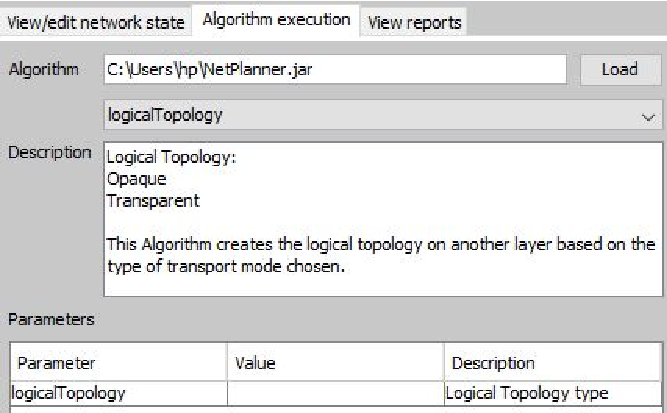
\includegraphics[width = 11cm]{Logical_Topology_Algorithm.pdf}
		\caption{Net2Plan Logical Topology Algorithm}
		\label{Logical_Topology_Algorithm}
	\end{figure}	
	
	There are two user defined parameters on this algorithm. The "logicalTopology" parameter defines the type of transport mode, Opaque or Transparent.\\
	
	%The other parameter, "maximumOpticalReach" is only needed for the Translucent transport mode to define the distance between OEO (Optical-Electrical-Optical) conversions.
	
	Besides creating this new Layer, the algorithm also copies the demands to that layer and defines the logical links based on the length of the physical ones.
	Figures \ref{Net2Plan_Opaque}, \ref{Net2Plan_Transparent}  demonstrate the resulting logical topologies for each transport mode.
	
			\begin{figure}[!h]
				\centering
				\subfigure[]{
					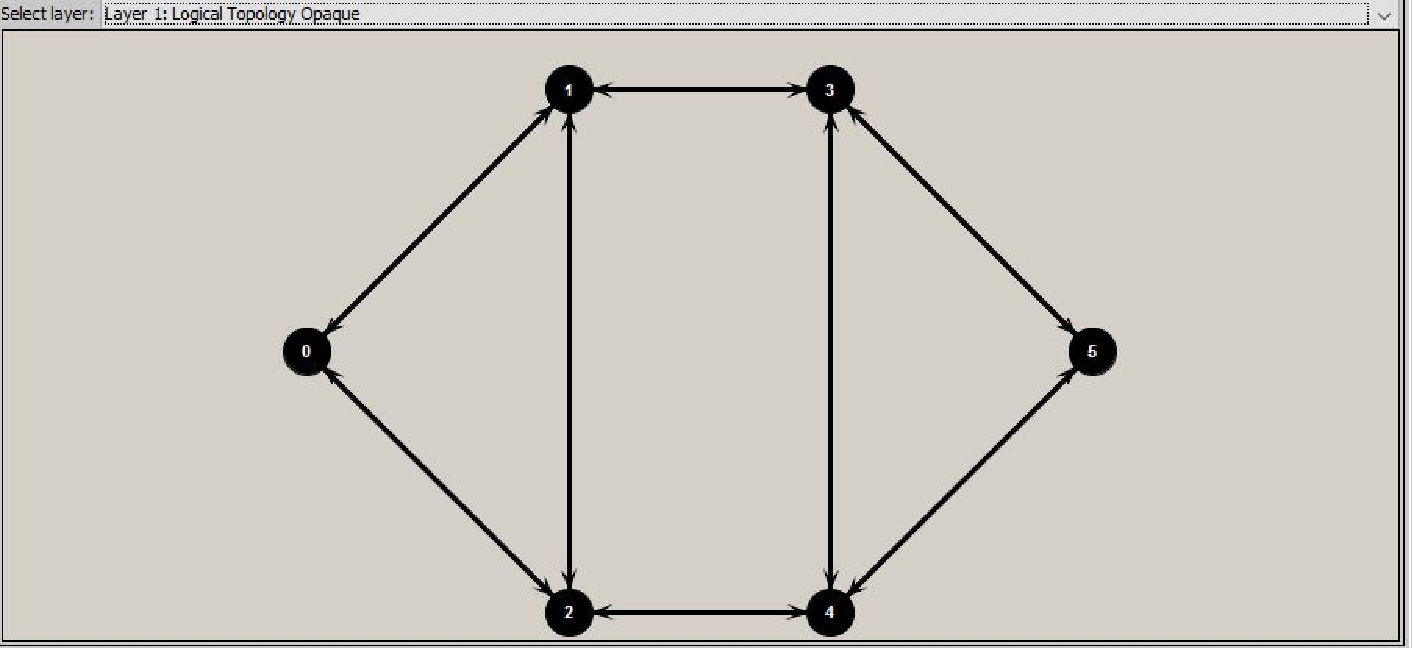
\includegraphics[width=7cm]{Net2Plan_Opaque.pdf}
					\label{Net2Plan_Opaque}					
				}
				\subfigure[]{
					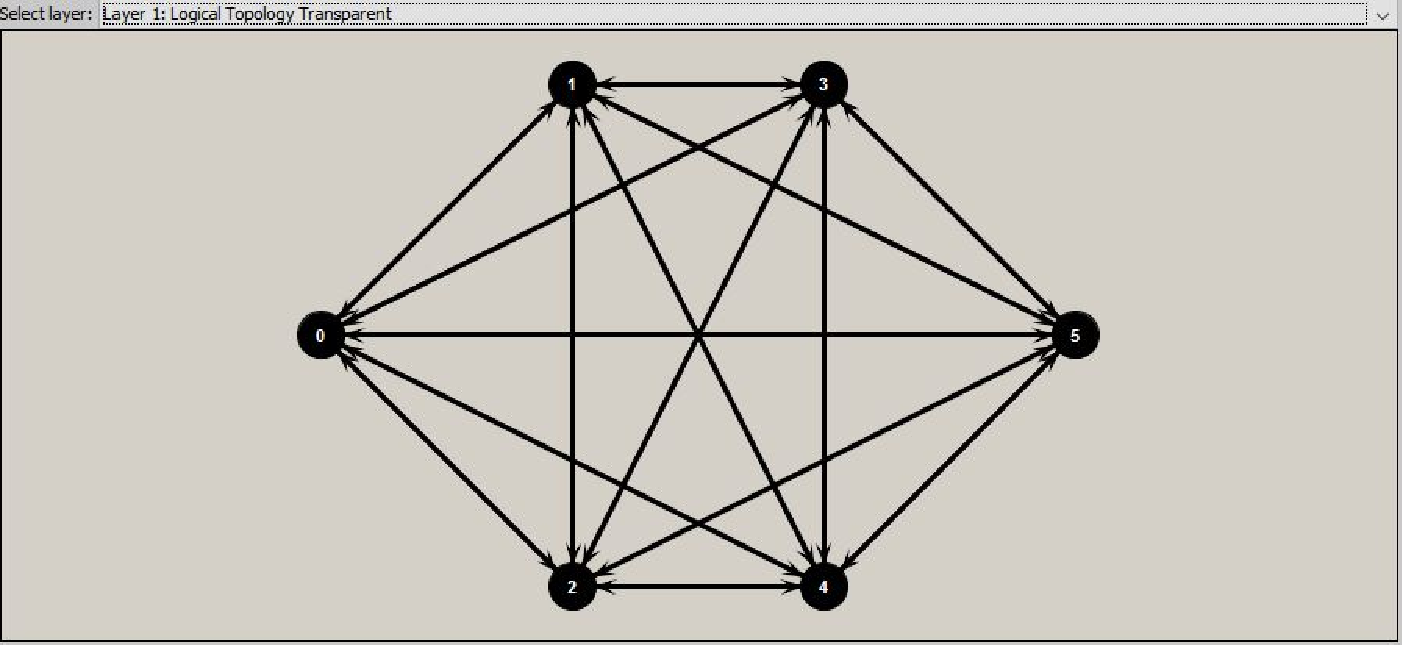
\includegraphics[width=7cm]{Net2Plan_Transparent.pdf}		
					\label{Net2Plan_Transparent}									
				}
				
				\caption{Logical Topology: a) Opaque; b) Transparent;}								
			\end{figure}	

	As can be seen on the logical topologies, for an Opaque transport mode the traffic goes through an OEO conversion at every node and as such the logical topology is the same as the physical one.
	
	In the Transparent mode, there are no regeneration in intermediate nodes and as such the logical topology shows that the traffic between nodes flows directly without grooming with signals from another source.
	
	%Lastly for the Translucent mode, the grooming is performed in a mix between the previous two modes. Up to a certain reach defined in the logical topology algorithm the network acts similarly to a transparent one and after that distance the signal is regenerated as in an Opaque network. For the example presented the optical reach was 400 km.
	\pagebreak
	\subsection*{Routing and Grooming} \label{Routing and Grooming}
	In this section, different routing and grooming options will be discussed for both a network without protection and using a 1+1 protection scheme (dedicated path protection).\\
	The routing will be done based on a shortest path algorithm where the routes for each demand are are created based one either the shortest number of hops needed to reach the destination node or by shortest distance in km. The option can be chosen as a user defined parameter on the algorithm as can be seen on Figure \ref{Grooming_Algorithm}. This algorithm does the routing in both the logical and physical topologies based on the transport mode chosen and makes sure routes are bidirectional meaning the route from node $o$ to $d$ should be the opposite direction of node $d$ to $o$ as there could be different routes with the shortest path that are not using the same path.
	
	\vspace{0.5cm}
	\begin{figure}[h!]
		\centering
		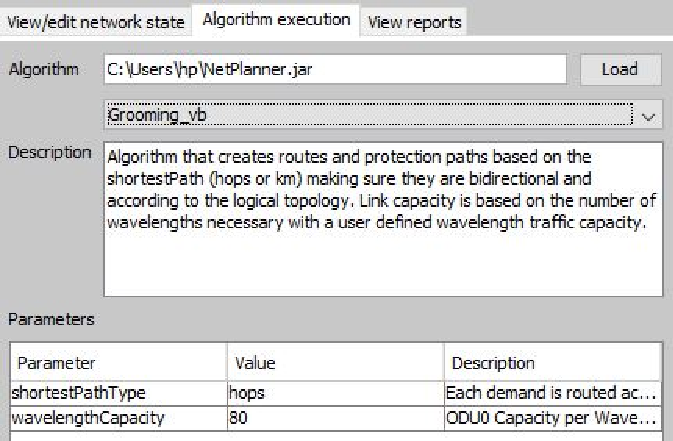
\includegraphics[width = 11cm]{Grooming_Algorithm.pdf}
		\caption{Net2Plan Grooming shortest Path Algorithm}
		\label{Grooming_Algorithm}
	\end{figure}	
	
	Besides the metric through which the shortest path is calculated, the other available parameter defines the amount of ODU0s each wavelength is capable of carrying. By default it is set for 80 ODU0s as it is equal to an ODU4 or 100 Gbit/s.\\

	%The other option for routing without protection is based on reducing the number of wavelengths needed for the network to carry all traffic. Instead of finding the shortest distance between origin and destination node, this algorithm creates the routes based on the previous ones, for example, if the first demand goes through a specific group of links and there is enough capacity in the wavelengths left for the traffic in the next one that demand will be routed to use this spare capacity instead of going through the shortest path.
	
	%As this algorithm is only trying to reduce wasted capacity in links the only user defined parameter available is as before the wavelength capacity in ODU0s, as can be seen on Figure \ref{Grooming2_Algorithm}. The default value is again defined as 80 ODU0s.
		
	%An important point to take into consideration in this algorithm is that even though it might reduce the number of wavelengths needed compared to the shortest path it is not the optimal solution. This fact is due to the limitation imposed by Net2Plan as there is not an option to obtain all available paths between two nodes. The option chosen in order to perform the calculations was to obtain two disjoint paths between the origin and destination node and then performs the steps explained above. This limitation is also felt when creating protection segments in the network as will be explained further on in the 1+1 protection scheme grooming.\\
	
    %\begin{figure}[h!]
	%	\centering
	%	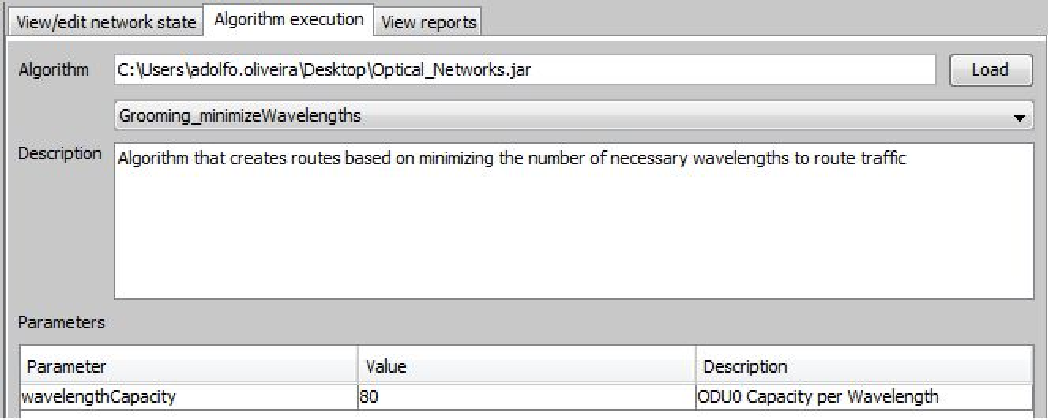
\includegraphics[width = 17cm]{Grooming2_Algorithm.pdf}
	%	\caption{Net2Plan  minimize wavelengths grooming Algorithm}
	%	\label{Grooming2_Algorithm}
	%\end{figure}	
	
	%To create the network routing with a 1+1 protection scheme in place, the algorithms developed for this instance are similar to the ones presented for a network without protection whereas in this case besides finding routes for each demand a protection segment is created with a disjoint path to the one used for the route. "Grooming1\_1" is an algorithm that creates the routes as in the "Grooming" algorithm by choosing the shortestPath and then making the disjoint path the protection one. This algorithm can be run as seen on \ref{Grooming11_Algorithm}.
	
	%\begin{figure}[h!]
	%	\centering
	%	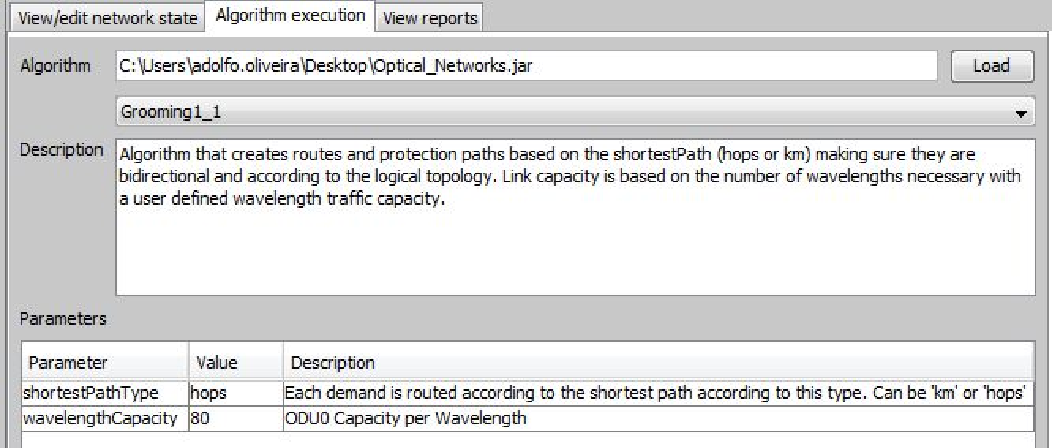
\includegraphics[width = 17cm]{Grooming11_Algorithm.pdf}
	%	\caption{Net2Plan Grooming with protection segments Algorithm}
	%	\label{Grooming11_Algorithm}
	%\end{figure}	
	
	The protection segments similarly to the routes have their own tab where information on their path, route it protects and such can be observed.

\newpage
	
	\subsection*{Reports} \label{Reports}
	As looking separately at each tab to obtain information for different parts of the network is a slow process and does not show some important metrics, Net2Plan allows for the creation of reports where in a similar way to algorithms they can be adjusted to display the information needed, these can also be seen in html format for an easier read. In this section, the report developed will be demonstrated.
	
%   	The first report developed for the optical network classes is called "lineMatrix". This report can be loaded as seen on Figure \ref{lineMatrix_Report}.
%	
%	\begin{figure}[h!]
%		\centering
%		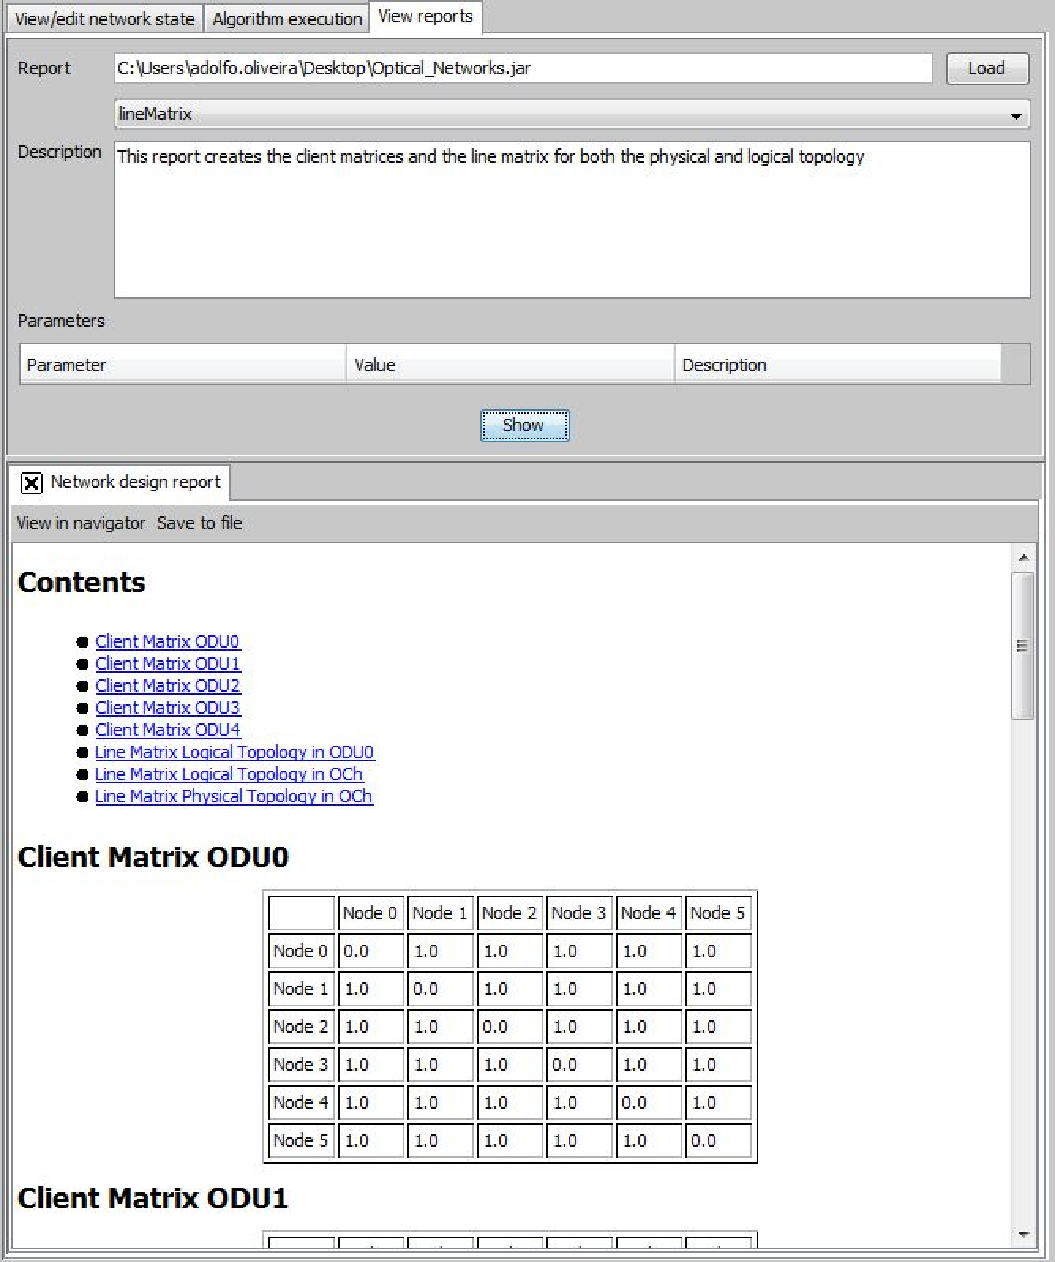
\includegraphics[width=15cm]{lineMatrix_Report.pdf}
%		\caption{Line matrix report}
%		\label{lineMatrix_Report}
%	\end{figure}
%	
%	This report showcases the client matrix created for each ODU type as well as the line matrices in both topologies. In the physical topology the matrix is in Och, number of wavelengths between nodes while on the logical topology there is both a matrix in Och and one in ODU0s.
%	
%	Another report that was created was called "simplifiedReport". This one is a simplified version of the "networkDesign" report whereas in this case only the most relevant information is displayed as can be seen on Figure \ref{simplified_Report}.
%	
%	\begin{figure}[h!]
%		\centering
%		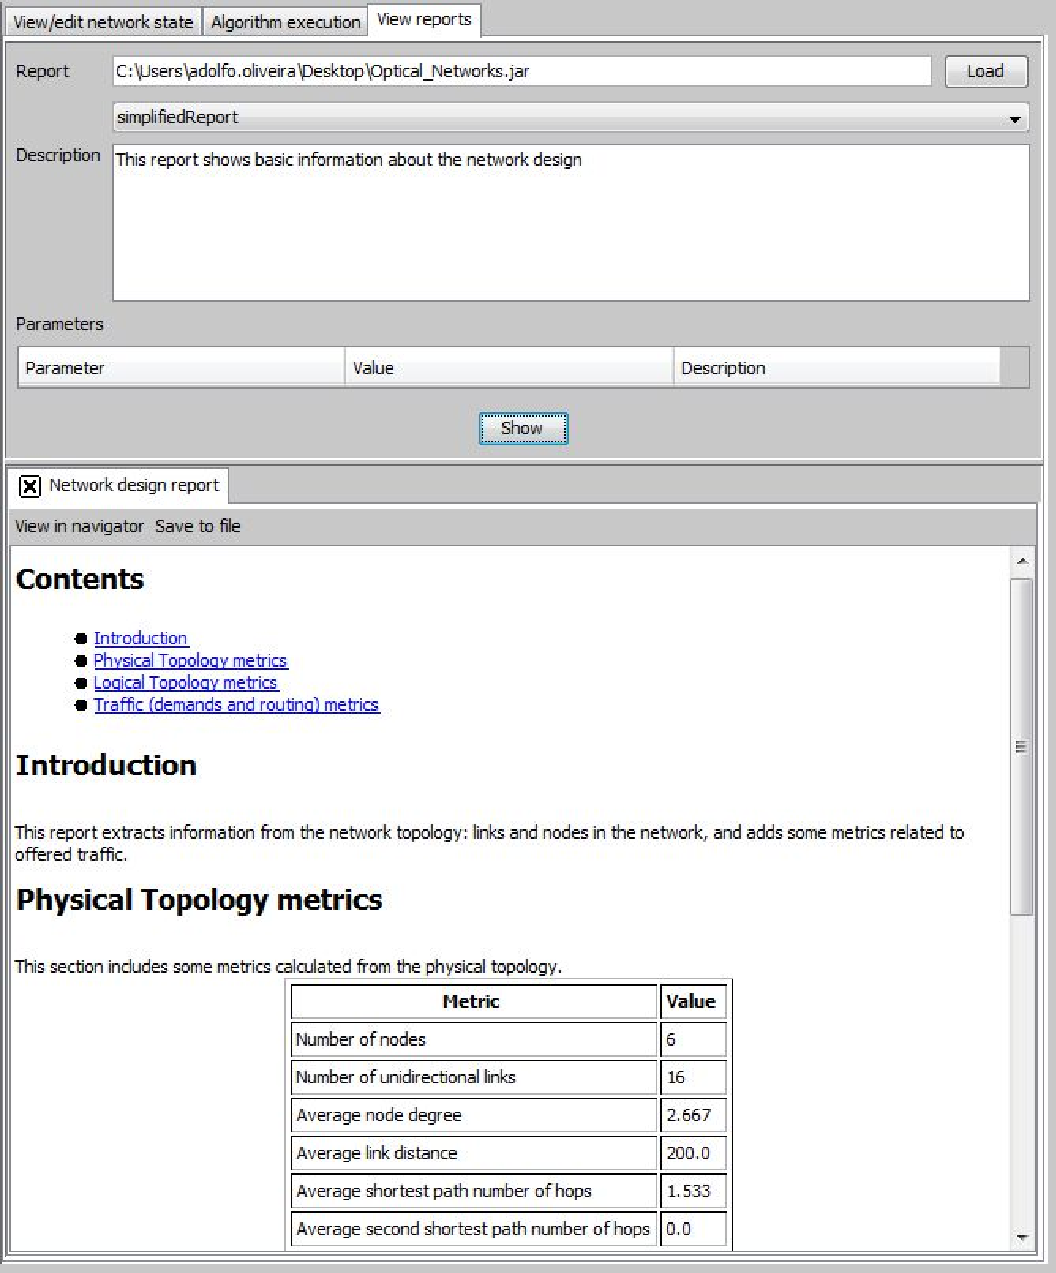
\includegraphics[width=16cm]{simplified_Report.pdf}
%		\caption{Simplified Report}
%		\label{simplified_Report}
%	\end{figure}	
%	
%	Both of these reports have no user defined parameters as they only relay network information. Another option to obtain more network metrics is to use the "Report\_networkDesignModified" as this is a modified version of the already built in Net2Plan report but with a few fixes. This option not only represents the metrics in tables but also has expressions indicating how some of the main network metric can be calculated from basic information. For example the average node degree is obtained by calculating $\frac{E}{N}$.\\
	
	A very important aspect in network planning that is not present natively in Net2Plan is a Network Cost report. To fulfil this gap, a report was created to obtain the network Capex based on user defined equipment costs present on Table \ref{EquipmentCosts}.
		
	\begin{table} [h]
		\centering
		\resizebox{0.4\textwidth}{!}{
		\begin{tabular} {|c|c|}
			\hline
			Equipment & Costs \\
			\hline
			OLT					&	15000\euro		\\ \hline
			Transponder			&	5000\euro/GB	\\ \hline
			Optical Amplifier	&	4000\euro		\\ \hline
			EXC					&	10000\euro		\\ \hline
			OXC					&	20000\euro		\\ \hline
			EXC Port			&	1000\euro/GB/s	\\ \hline
			OXC Port			&	2500\euro/port	\\ \hline										
		\end{tabular}}
		\caption{Equipment Costs}			
		\label{EquipmentCosts}			
	\end{table}
	
	These Equipment costs are introduced into a report as user defined parameters as can be seen on Figure \ref{networkCost_Report}.
	
	\begin{figure}[h!]
		\centering
		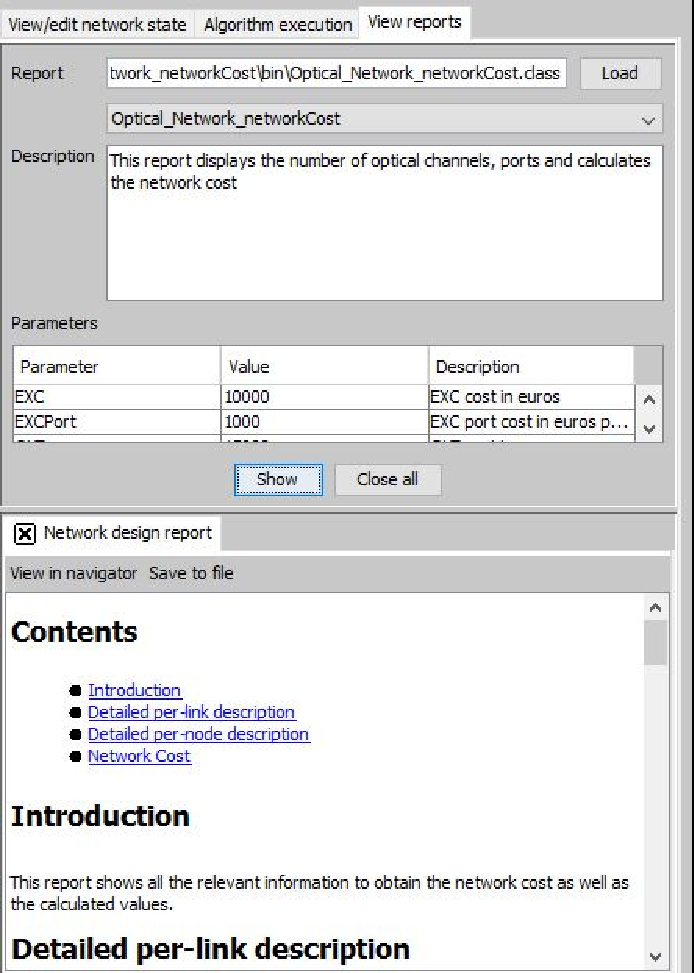
\includegraphics[width=7.5cm]{networkCost_Report.pdf}
		\caption{Network Cost Report}
		\label{networkCost_Report}
	\end{figure}	
	
	Besides the equipment costs, this report also has the parameter "span". The value of this variable is used to calculate the number of optical amplifiers needed in the network using Equation \ref{amplifiersLink}.
	
	\begin{equation}
		N^R = \sum\limits_{l=1}^L\left(\left\lceil\frac{len_l}{span}\right\rceil-1\right)
		\label{amplifiersLink}
	\end{equation}

	The other parameters of this equation being:
	
	\begin{itemize}
		\item{$N^R$			$\rightarrow$ Total number of regenerators/amplifiers}
		\item{$len_l$		$\rightarrow$ Length of link l}
		\item{$span$		$\rightarrow$ Distance between amplifiers}	
	\end{itemize}	
	
	By running the report three main categories are presented to the user.
	
	The first category displayed by the report is the Detailed per-link description. In here the number of optical channels or wavelengths is displayed for each link based on the grooming algorithm used. The numbers displayed are based on the physical topology and represent all the wavelengths that will be needed to transport the network traffic. Using this information it is possible to obtain the average and total number of optical channels on the network.
	
	Besides the number of wavelengths, this section also indicates the amount of amplifiers necessary in each link. \\
	
	The second category is the Detailed per-node description. This section displays a table indicating how many ports are needed of each type for every node. The number of tributary ports obtained in each node is the sum of all traffic originating from that node or ending on it depending if its the input or output ports divided by the amount of traffic each optical channel can carry. This number also depends on the links through which traffic will be routed, for example, if 40 ODU0s are transmitted into 2 separate links only one wavelengths could carry it but as they are going through different routes then 2 wavelengths will be used resulting in also a need for 2 tributary ports.\\
	
	The number of line ports is obtained by adding the total amount of optical channels in the links that use that specific node as origin or destination.\\
	
	Finally the total number of ports is as expected the sum of all the tributary ports with the line ones. With this information the average and the total number of ports in the network can be obtained which will later be used in calculating the network cost.\\
	
	Having the node and link information available, the network cost can then be calculated as displayed on the third category of the report.								
	The Node electrical cost is obtained with Equation \ref{electricalPortsCostTransparent} for a Transparent Network.
	
	\begin{equation}
		C_{exc} = \left(\gamma_{e0}\times N\right) + \left(\gamma_{e1} \times \tau \times 2 \times P_{TRIB}\right)
		\label{electricalPortsCostTransparent}
	\end{equation}
	
	\begin{itemize}
		\item{$C_{exc}$		$\rightarrow$	Electrical Ports Cost}
		\item{$\gamma_{e0}$	$\rightarrow$	EXC cost in Euros}
		\item{$N$			$\rightarrow$	Number of Nodes}
		\item{$\gamma_{e1}$	$\rightarrow$	EXC port cost in Euros per GB/s}
		\item{$\tau$		$\rightarrow$	Traffic supported by optical channel}
		\item{$P_{TRIB}$	$\rightarrow$	Number of tributary ports}
	\end{itemize}
	
	The cost values can be obtained from Table \ref{EquipmentCosts}, the number of nodes is a known value when designing a network, the traffic supported by optical channel is defined by the grooming algorithm or by dividing the link capacity by its amount of optical channels and the number of tributary ports was obtained on the previous section of the report. \\
	
	For an Opaque network, the electrical nodes cost is similar as displayed in Equation \ref{electricalPortsCostOpaque}.\\
	
	\begin{equation}
	C_{exc} = \left(\gamma_{e0}\times N\right) + \left(\gamma_{e1} \times \tau \left(P_{LINE} + P_{TRIB}\right)\right)
	\label{electricalPortsCostOpaque}
	\end{equation}	\\
	
	The node optical cost on the other hand, can be calculated for a Transparent network using Equation \ref{opticalPortsCost}.
	
	\begin{equation}
		C_{oxc} = \left(\gamma_{o0} \times N \right) + \gamma_{o1} \times  \left(P_{LINE} + P_{TRIB}\right)
		\label{opticalPortsCost}
	\end{equation}	
	
	\begin{itemize}
		\item{$C_{oxc}$		$\rightarrow$	Optical Ports Cost}
		\item{$\gamma_{o0}$	$\rightarrow$	OXC cost in Euros}
		\item{$N$			$\rightarrow$	Number of Nodes}
		\item{$\gamma_{o1}$	$\rightarrow$	OXC port cost in Euros}
		\item{$P_{TRIB}	$	$\rightarrow$	Number of tributary ports}
		\item{$P_{LINE} $	$\rightarrow$	Number of line ports}
	\end{itemize}
		
	As for the electrical ports, the cost values were previously defined in Table \ref{EquipmentCosts} and as such, only the number of ports is needed. These value were obtained on the second part of the report (Detailed per-Node description). \\
	
	For an Opaque network, the node optical cost is 0 as the ports are all electrical. \\
	
	The Node Total Cost is as expected the sum of both the optical and electrical node costs. \\
	
	The rest of the network cost is from the links. This cost is obtained with Equation \ref{linksCost}.
	
	\begin{equation}
		C_L = \left(\gamma_0^{OLT} \times L\right) + \left(\gamma_1^{OLT} \times \tau \times W\right) + \left(N^R \times c^R\right)
		\label{linksCost}
	\end{equation}	
	
	\begin{itemize}
		\item{$C_L$				$\rightarrow$	Links Cost}
		\item{$\gamma_0^{OLT}$	$\rightarrow$	OLT cost in Euros}
		\item{$L$				$\rightarrow$	Number of unidirectional Links}
		\item{$\gamma_1^{OLT}$	$\rightarrow$	Transponder cost in Euros}
		\item{$\tau$			$\rightarrow$	Traffic per port}
		\item{$W$				$\rightarrow$	Total number of optical channels}
		\item{$N^R$				$\rightarrow$	Total number of optical amplifiers}
		\item{$c^R$				$\rightarrow$	Optical amplifiers cost in Euros}
	\end{itemize}
	
	As in previous equations, the costs are all available in Table \ref{EquipmentCosts}. The total number of optical channels can be obtained by summing the wavelengths in each link on the Detailed per-Link description section. The number of optical amplifiers was calculated previously with Equation \ref{EquipmentCosts}.
	
	The middle part of the equation: $\gamma_1^{OLT} \times \tau \times W$ refers to the Transponders cost while the rest is the "Fiber" and the "OLT" cost.	Lastly the total network cost can be obtained by adding the Links cost with the Nodes cost.\\
	
	\section*{Results}
	This section will display the results obtained using the algorithms and reports previously explained for a network with an Opaque transport mode and for one with Transparent.

	
	\subsection*{Opaque with 1+1 protection}
	%For this case, the difference to the previous example will be as for the case of a transparent network in the creation of a protection segment for each route.
	
	The results will be displayed only in the logical topology as in an opaque network it is the same as the physical one.
	Using the algorithm presented on figure \ref{Grooming_Algorithm} the routes and protection segments are created as well as the grooming. \\
	
	There is not a second algorithm type for wavelengths reduction due to the fact that, that algorithm chooses the best path based on the shortest or disjointed path which in this case both need to be used one for work and one for protection. As such, is difficult to reduce in any instance the shortest path because of the algorithm performance.
	
	The traffic matrix for the reference 6 node network, used for demonstration is shown below.
	
	\begin{figure}[h!]
		\centering
		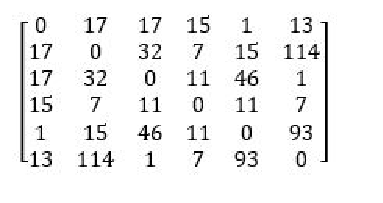
\includegraphics[width=9cm]{opaqueLineMatricesLogical11.pdf}	
		\caption{}
		\label{opaqueLineMatricesLogical11}								
	\end{figure}	
	
	The amount of traffic that needs to be reserved in each link is as was to be expected a lot higher due to the need to reserve double the amount and in more links. The same happens in terms of wavelengths. \\
	
%	Tab layer will display the average number of hops per protection segment as in this case as the other metrics will stay the same. This is shown on Figure \ref{simplifiedReportOpaque11}.
%	
%	\begin{figure}[h!]
%		\centering
%		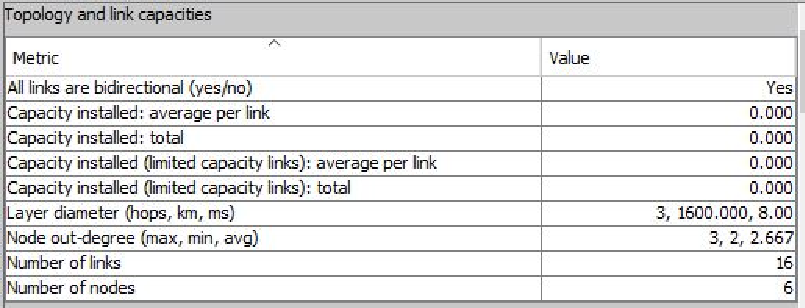
\includegraphics[width=9cm]{simplifiedReportOpaque11.pdf}	
%		\caption{simplified Report for opaque transport mode with 1+1 protection}
%		\label{simplifiedReportOpaque11}								
%	\end{figure}
%	
%	The number obtained for the second shortest path is the same as was obtained in the physical topology in the transparent network since as explained the algorithm being used is the same only difference will be on the way the grooming is done. \\
	
	The number of wavelengths can again be seen on the links section of the "networkCost" report as well as the amplifiers needed on Figure \ref{networkCost_Report_Links_Opaque11}.
	
	\begin{figure}[h!]
		\centering
		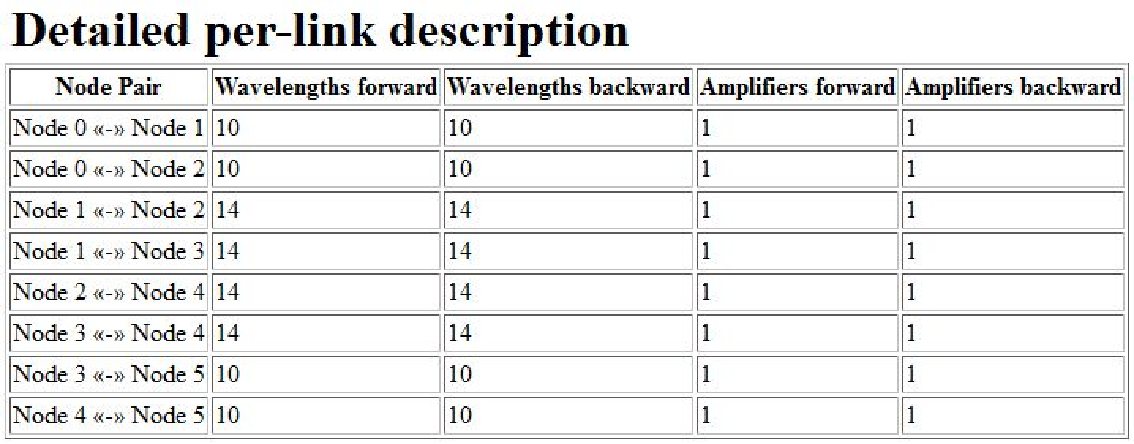
\includegraphics[width=11cm]{networkCost_Report_Links_Opaque11.pdf}	
		\caption{Links for Opaque Network with 1+1 Protection}
		\label{networkCost_Report_Links_Opaque11}								
	\end{figure}	
	
	The conclusions to take from these results are the same as was previously discussed as the number of amplifiers does not change and the wavelengths are the ones shown on the line matrices.
	
	As for the nodes in the network Figure \ref{networkCost_Report_Nodes_Opaque11} shows the ports needed.
	
	\begin{figure}[h!]
		\centering
		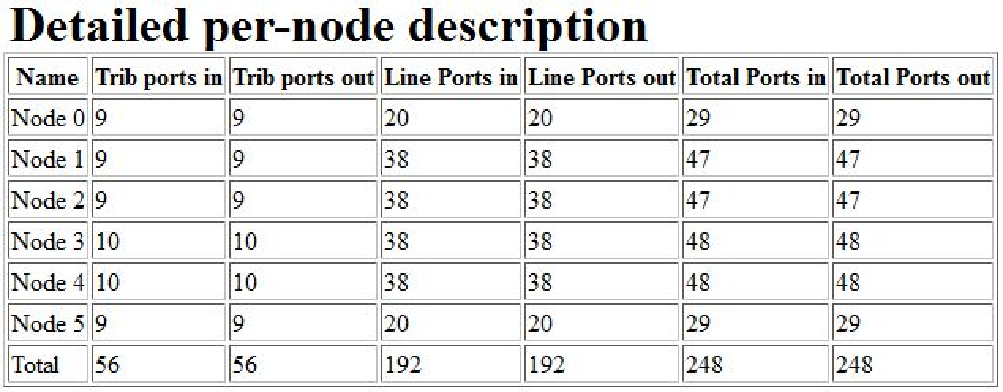
\includegraphics[width=11cm]{networkCost_Report_Nodes_Opaque11.pdf}	
		\caption{Nodes for Opaque Network with 1+1 Protection}
		\label{networkCost_Report_Nodes_Opaque11}								
	\end{figure}		
	
	Again, the difference for the case without protection is only on the number of line ports as this value is based on the number of wavelengths going in or out of that node.
	
	Comparing the number of ports obtained here with the network with a transparent transport mode, the amount is lower for the opaque network due to the reduced number of wavelengths required to route the traffic. \\
	
	Lastly the total network cost is on Figure \ref{networkCost_Report_Cost_Opaque11}.\\
	
	\begin{figure}[!h]
		\centering
		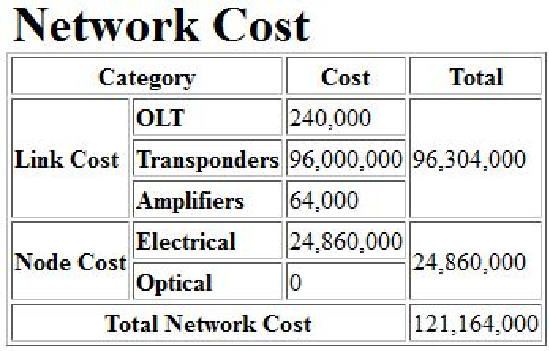
\includegraphics[width=9cm]{networkCost_Report_Cost_Opaque11.pdf}	
		\caption{Network Cost for Opaque Network with 1+1 Protection}
		\label{networkCost_Report_Cost_Opaque11}								
	\end{figure}	
	
	\pagebreak
	
	The increase in cost is as described on the transparent network just based on the additional number of wavelengths required which translates in also more trunk ports needed. As noted above in the amount of ports, the cost is also lower in this instance when compared to the transparent network due to the cheaper cost in transponders and optical ports.
	
	
	
		\subsection*{Transparent with 1+1 protection}
		
		
		For a network with a transparent transport mode, the routing as was explained before, is done using a shortest path algorithm since there are no traffic grooming between different node pairs. For this instance as there is also a 1+1 protection scheme in place, the algorithm needs to not only create the routes but also a protection segment for each route. This segment is the shortest disjoint path of the route created.

		
		Comparing the results obtained here with the previous example, it can be seen that the amount of traffic and wavelengths is significantly higher. It is in both cases, double the amount of before since the same quantity needs to be reserved for protection.\\
		

		
		The conclusions that can be taken from the physical topology are as explained before, the huge number of wavelengths is related to the needed for double the amount of traffic where this extra will go through even more links.
		
		For the logical topology the Average second shortest path number of hops is 1 since as for the shortest path, it is considered that there are always direct links between nodes in a transparent network. As for the physical topology, this value is not so obvious as it has to be calculated based on the second shortest path between each node pair. \\
		
			
	
			
		These differences for the transparent network with protection segments can also be seen on the information provided in the "networkCost" report. Figure \ref{networkCost_Report_Links_Transparent11} shows the results for the links in the physical topology.\\
		
		\begin{figure}[!h]
			\centering
			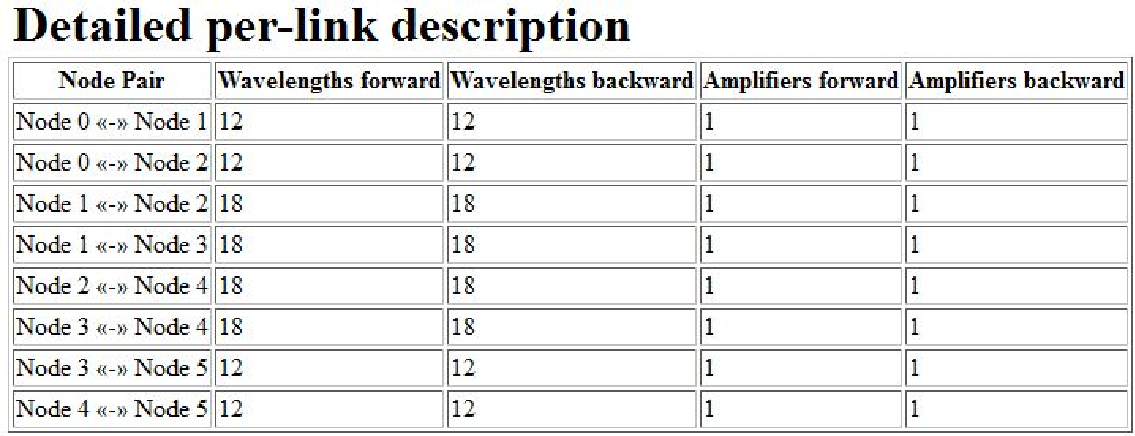
\includegraphics[width=11cm]{networkCost_Report_Links_Transparent11.pdf}
			\caption{Links for Transparent Network with 1+1 Protection}
			\label{networkCost_Report_Links_Transparent11}						
		\end{figure}	
		
		It can be seen that as expected the number of amplifiers is the same due to the link lengths remaining constant but the number of wavelengths are higher due to having a grooming scheme worst with this topology.\\
		\newpage
		The results in terms of ports per node are shown below.
		
		\begin{figure}[!h]
			\centering
			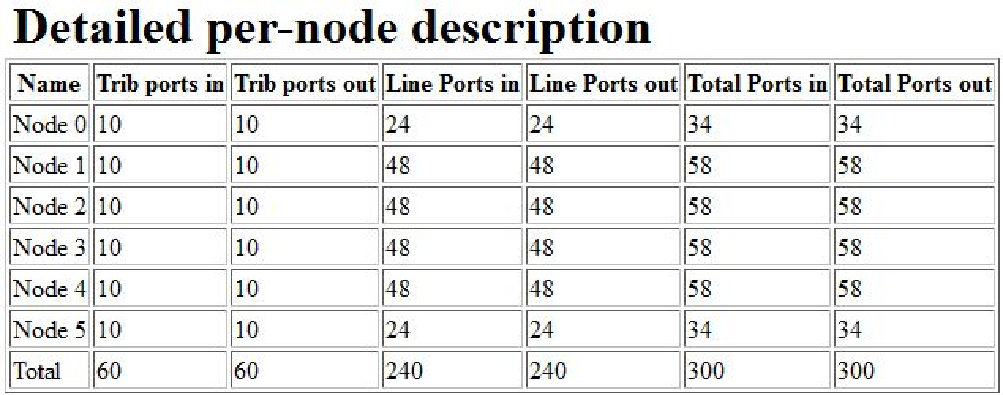
\includegraphics[width=11cm]{networkCost_Report_Nodes_Transparent11.pdf}
			\caption{Nodes for Transparent Network with 1+1 Protection}
			\label{networkCost_Report_Nodes_Transparent11}						
		\end{figure}
		
		 The number of tributary ports remain the same but the number of line ports increase based on the higher number of wavelengths needed in the network.\\
		
		Lastly, the total network cost is shown on Figure \ref{networkCost_Report_Cost_Transparent11}.\\
		
		
		\begin{figure}[!h]
			\centering
			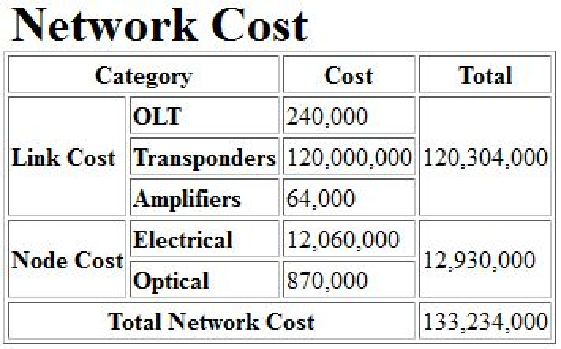
\includegraphics[width=9cm]{networkCost_Report_Cost_Transparent11.pdf}	
			\caption{Network Cost for Transparent Network with 1+1 Protection}
			\label{networkCost_Report_Cost_Transparent11}								
		\end{figure}		
		
		The results obtained for the network Cost confirm those obtained in the previous categories in this report. The OLT and amplifiers cost does not change as the number of links and amplifiers remains the same. Similarly, the electrical ports cost is also the same as the amount of ADD/DROP ports remains the same.
		
		The differences are in the Transponders cost in the links and the Optical cost in the nodes. These as expected, cost more based on the increased number of them needed in the network to have a 1+1 protection scheme in a transparent transport mode network.
		
	
	\newpage
	
	
	\section*{Simulations}
	To access the Simulations window go to  "Tools $\rightarrow$ Online Simulation" or press $Alt + 3$. The simulations menu is very similar to the one available for network design with the notable difference that in this instance the network needs to have already been saved with every definition done as all the tabs described earlier are only available here for viewing.
	
	Using the already built network with the demand set introduced as well as routing and protection segments, an example of a Time-varying simulation is demonstrated. The main parameters to be chosen on this simulation are the "Event generator" and the "Provisioning algorithm", displayed on Figures \ref{Net2Plan_Simulation} and \ref{Net2Plan_Simulation_1}.
	
	\vspace{-0.3cm}
	
	\begin{figure}[!h]
		\centering
		\subfigure[]
		{
			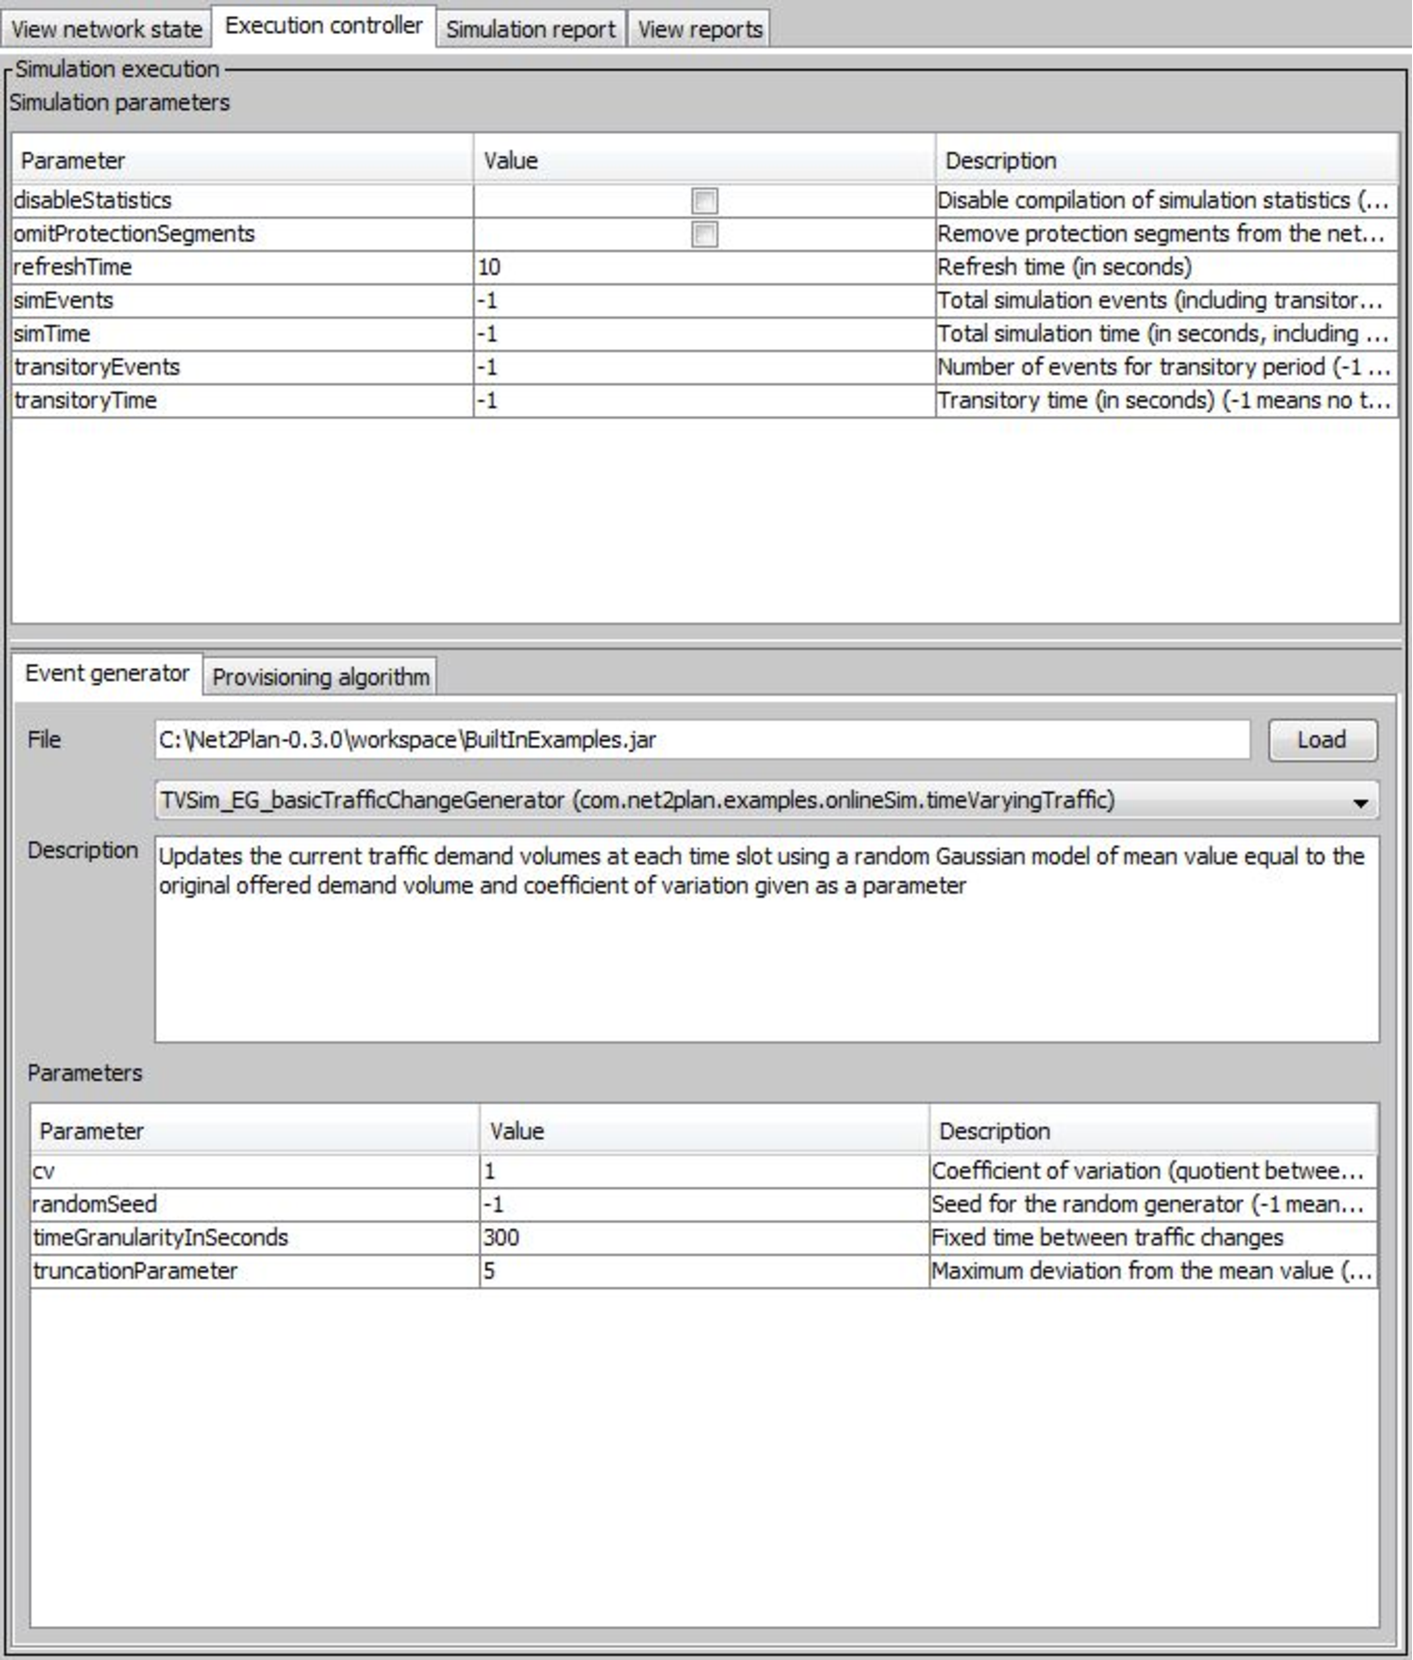
\includegraphics[width = 5cm]{Net2Plan_Simulation.pdf}
			\label{Net2Plan_Simulation}
		}
		\subfigure[]
		{
			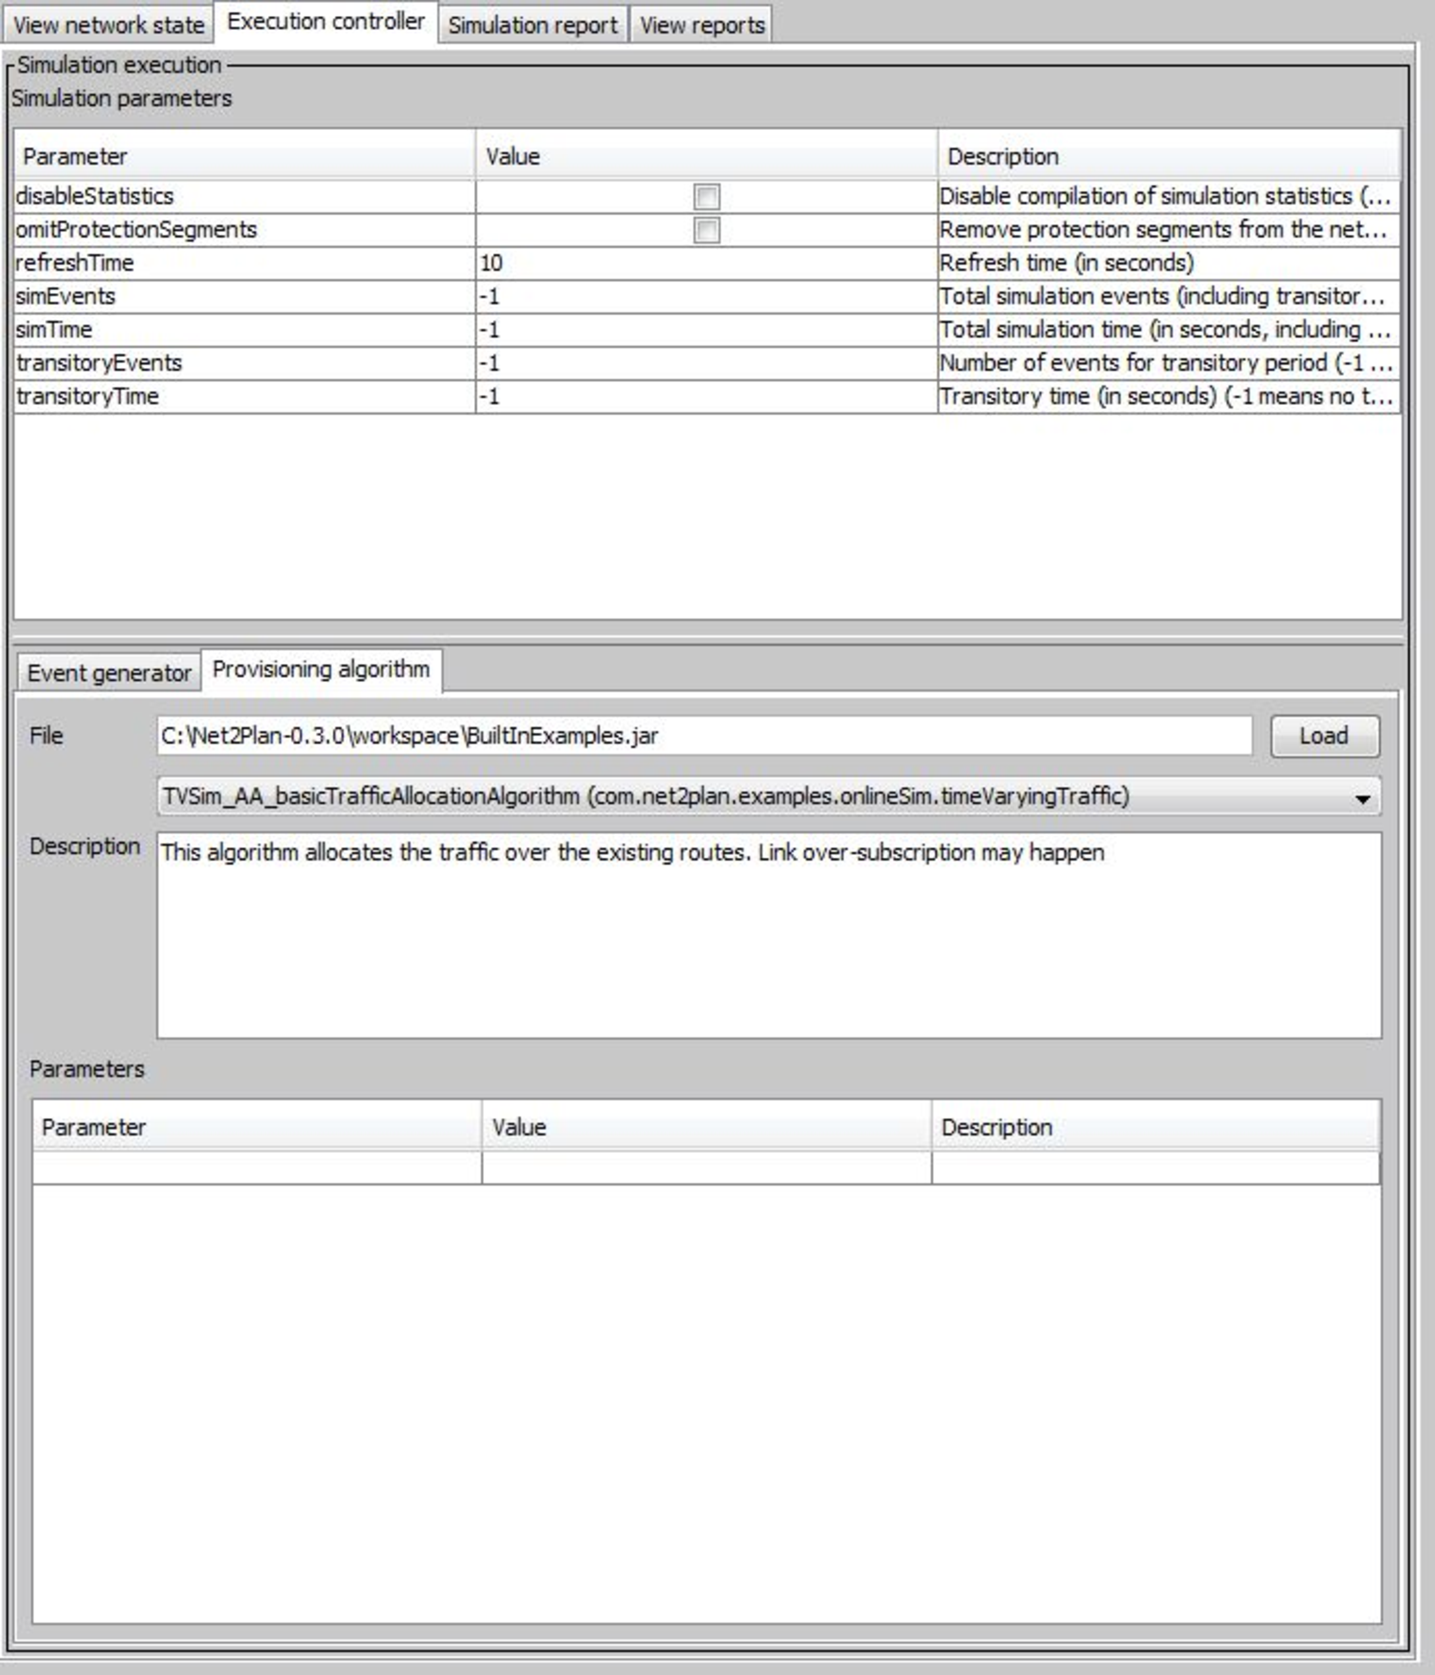
\includegraphics[width = 5cm]{Net2Plan_Simulation_1.pdf}
			\label{Net2Plan_Simulation_1}
		}
		\caption{a) Net2Plan Event generator ; b) Net2Plan Provisioning algorithm}
	\end{figure}	

	The Event generator shown creates a time varying simulation by updating the network traffic based on the chosen parameters while the allocation algorithm in this case only allocates this traffic into the available routes. Besides these options it is also possible to change the main simulation parameters which are displayed on the top half.

	Having defined all the simulation parameters and the other necessary options, the simulation can be started by just pressing "run" below the network topology at the lower left side. The "simulation controller" will update automatically based on the time defined at the simulation parameters or it can be paused for an update on the results.
	
	\newpage

	\section*{Implementing new algorithms on Net2Plan}
	\vspace{1cm}
	This section will demonstrate some of the possibilities provided by Net2Plan as an open source tool. By creating new algorithms or reports it is possible to adapt this program for most necessities in terms of network planning.

	There are already several built-in algorithms present in Net2Plan but as it is impossible to have an algorithm built for every specific necessity it is possible for each user to build new ones or modify existing ones to fulfil what needs to be done.\\
	
	As everything in Net2Plan was built in Java, the program "Eclipse" that can be downloaded from \url{https://eclipse.org/downloads/} was chosen as the best option for coding. All the .java files from the available algorithms in Net2Plan can be downloaded from its website and introduced into "Eclipse" to create a class.
	
	When opening Eclipse, the first choice is to define the work directory in which all the projects will be created. Having defined the workspace, Figure \ref{Eclipse_project} demonstrates the window for creating new projects in Eclipse, this can be accessed by going into "File $\rightarrow$ New $\rightarrow$ Java Project". In this window, only the name needs to be defined and then finish.
	
	\vspace{1.5cm}
	\begin{figure}[h!]
		\centering
		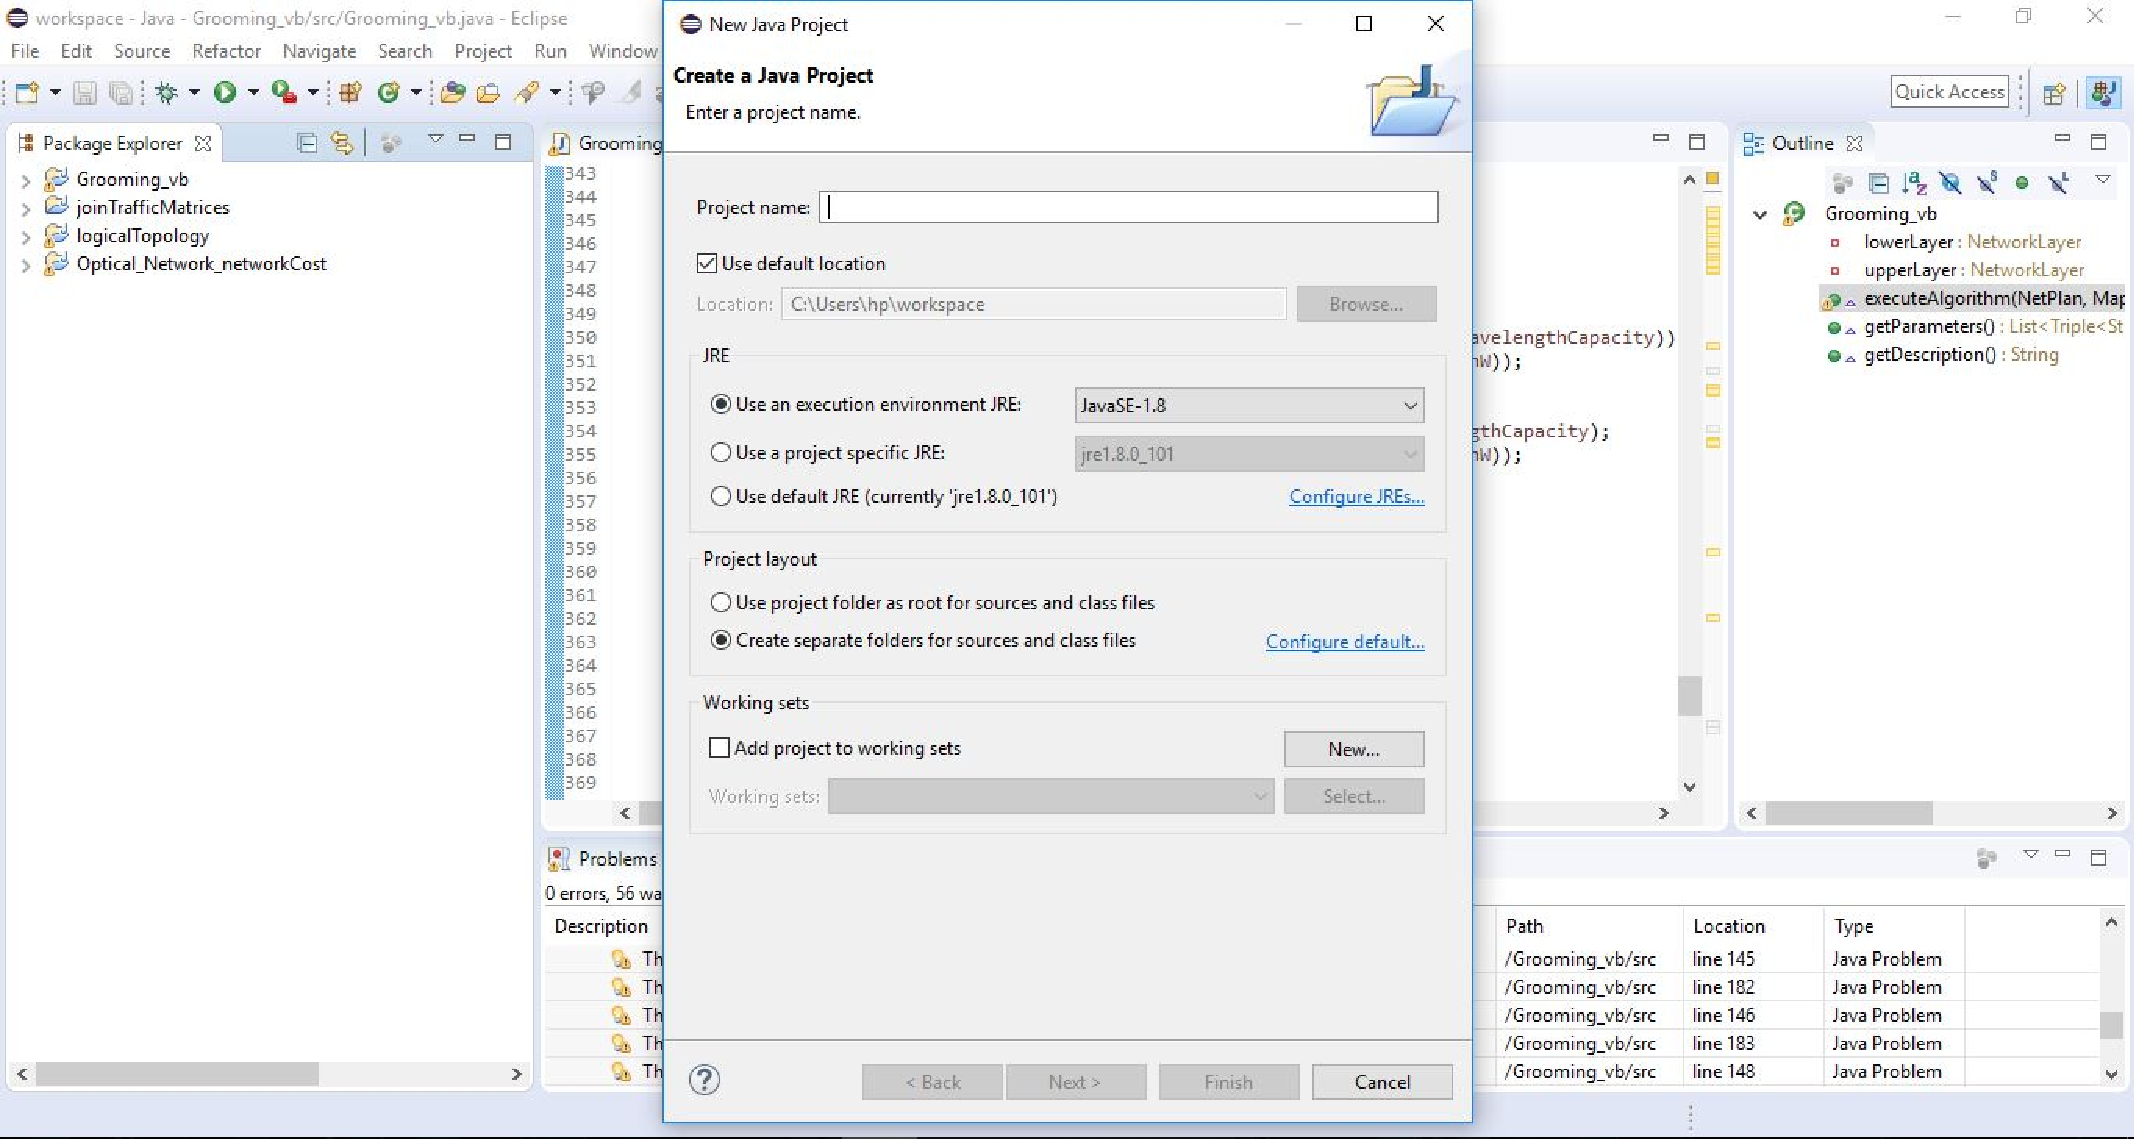
\includegraphics[width = 13cm]{Eclipse_project.pdf}
		\caption{Eclipse new project}
		\label{Eclipse_project}
	\end{figure}	
	
	\newpage
	
	Having created a new project, a "src" directory should be available where the .java should be located. As a starting point, an existing algorithm should be used as a template and then modified to do its necessary purpose. Figure \ref{Eclipse_project_1} shows a newly created project called "logicalTopology".
	
	\vspace{1.5cm}
	\begin{figure}[h!]
		\centering
		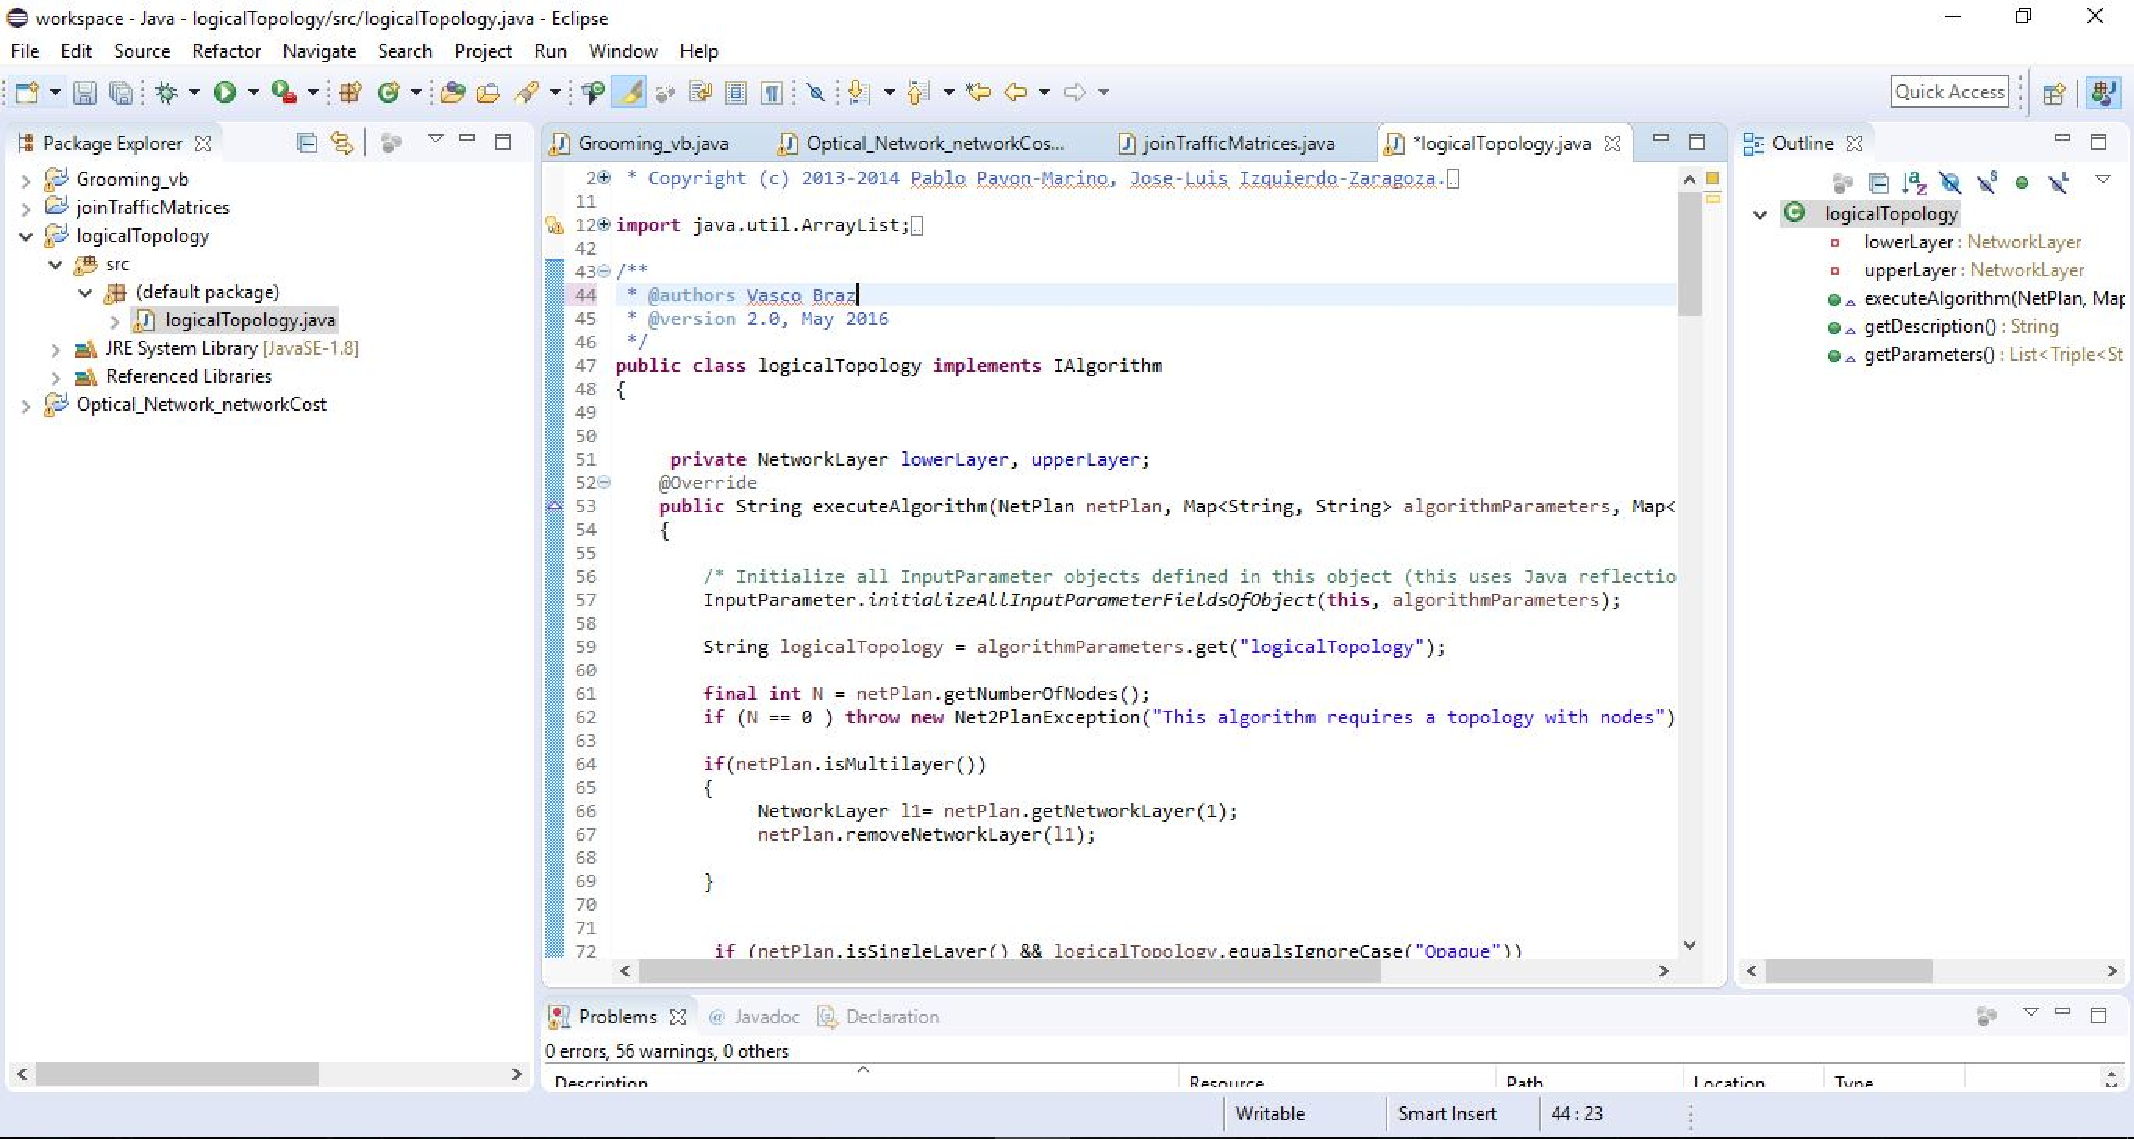
\includegraphics[width = 13cm]{Eclipse_project_1.pdf}
		\caption{Eclipse new project with source file}
		\label{Eclipse_project_1}
	\end{figure}	
	
	To add the library files to a project, right click on it and choose "Build Path $\rightarrow$ Configure Build Path ..." . On the window that appears, press "Add External Jars..." and include all the files in the Net2Plan "lib" directory as shown on Figures \ref{Eclipse_libraries} and \ref{Eclipse_libraries_1}.
	
	\vspace{1.5cm}
	\begin{figure}[!h]
		\centering
		\subfigure[]
		{
			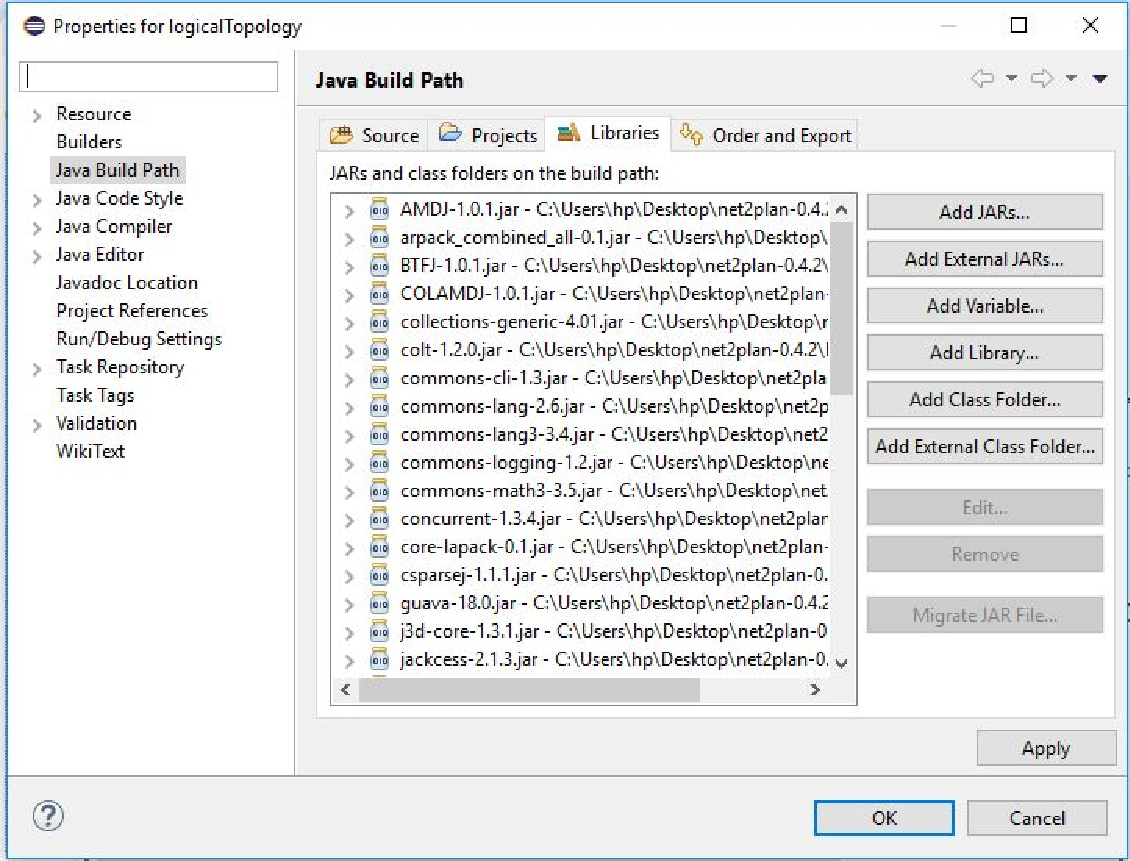
\includegraphics[width = 7.2cm]{Eclipse_libraries.pdf}
			\label{Eclipse_libraries}
		}
		\subfigure[]
		{
			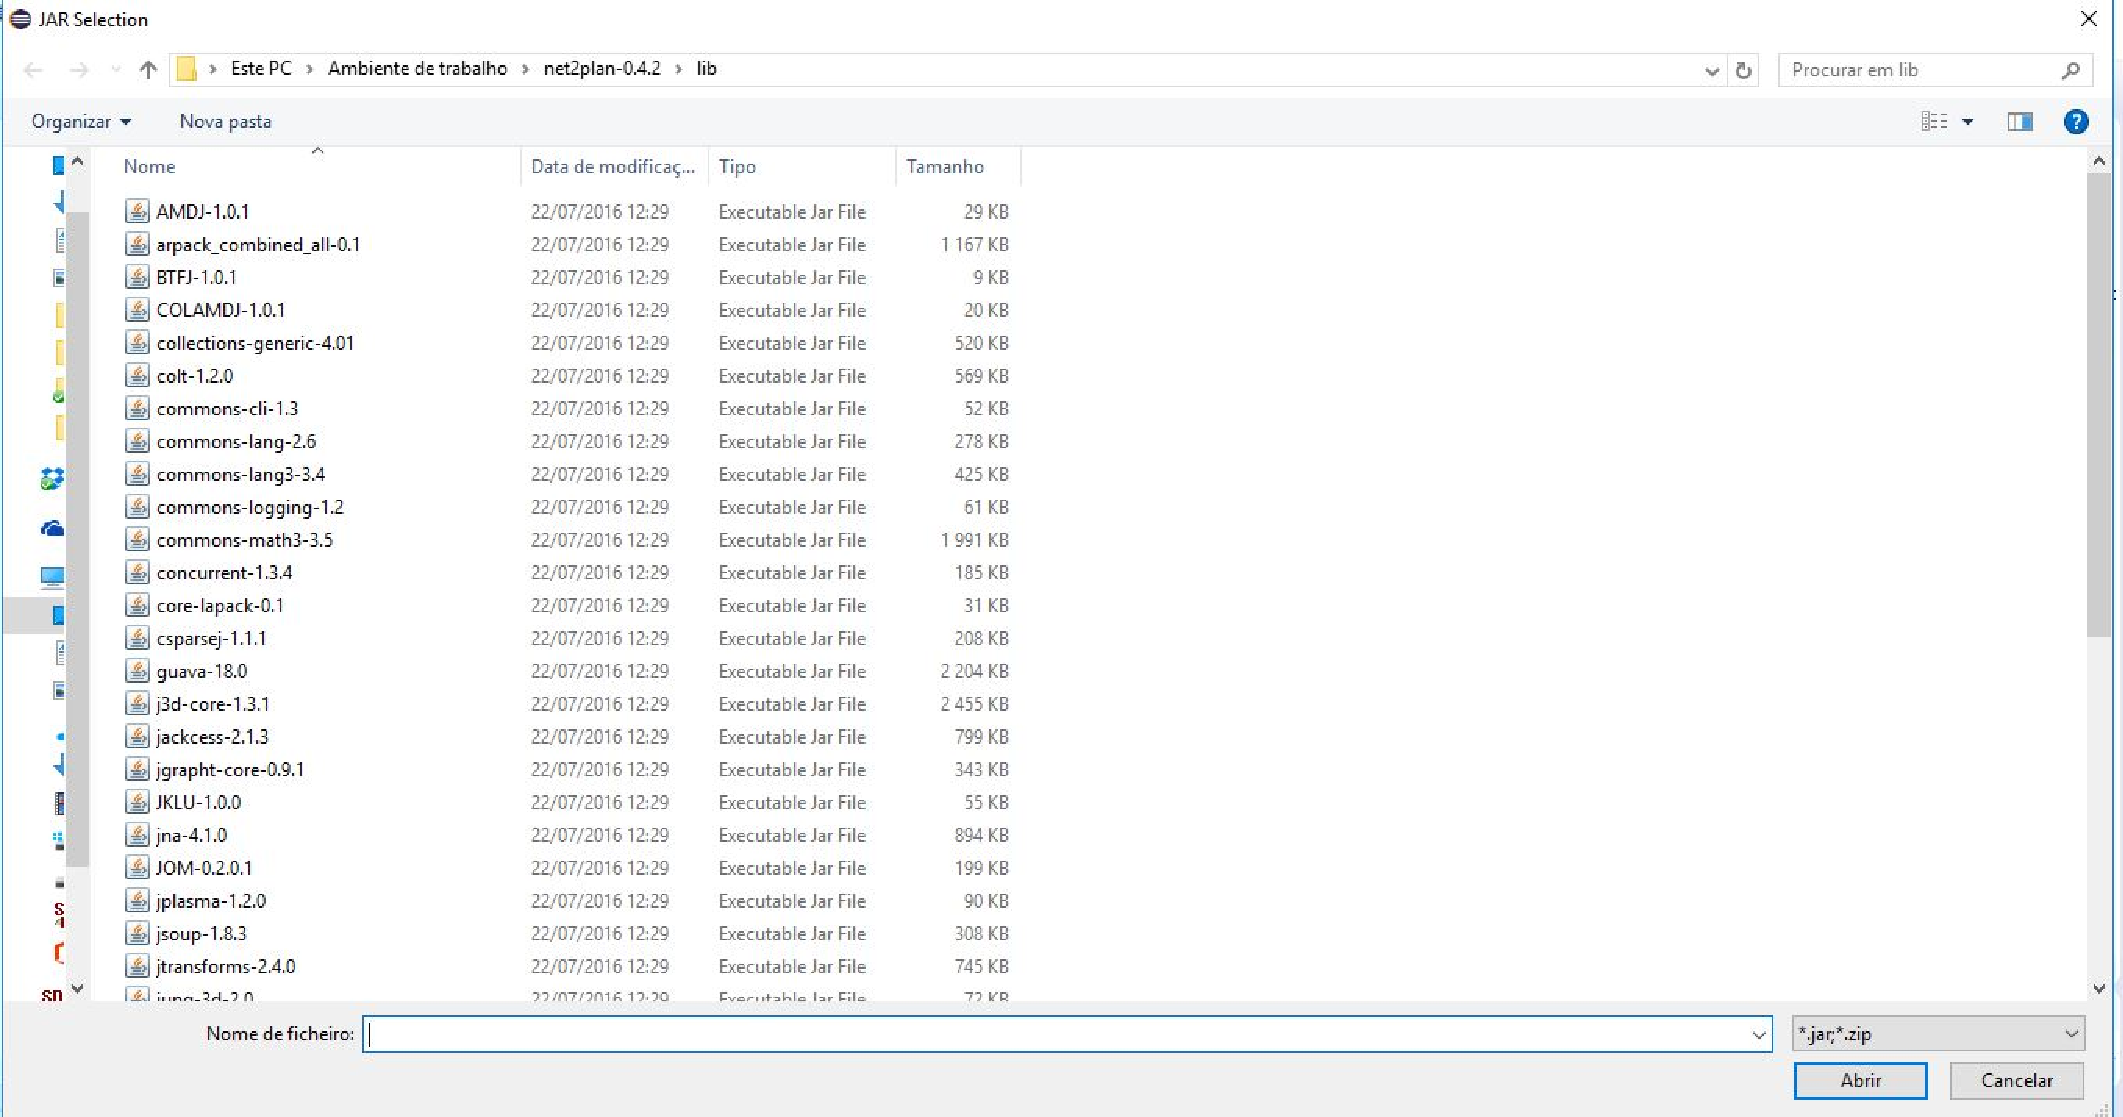
\includegraphics[width = 8.2cm]{Eclipse_libraries_1.pdf}
			\label{Eclipse_libraries_1}
		}
		\caption{a) Eclipse Java Configure Build Path ; b) Net2Plan library files}
	\end{figure}	
	

	
	To further illustrate how these modifications to algorithms work, the project created above using an existing code as a template was modified to create a new algorithm which creates the logical topology of a network in another layer.
	\newpage
	 The code created is shown on Figure \ref{Eclipse_project}.
	By saving this project on Eclipse a .class file is created on the bin directory of the project which can be loaded on Net2Plan. On the "Algorithm execution" tab at the "Offline network design", the "BuiltInExamples.jar" is loaded as the default location for algorithms and as it is a .jar file all the available ones that came with Net2Plan are integrated into it.	To get the newly created algorithm available, press "Load" and find the .class file created in Eclipse as shown on Figure \ref{Net2Plan_introduce_algorithm}.
	
	\begin{figure}[h!]
		\centering
		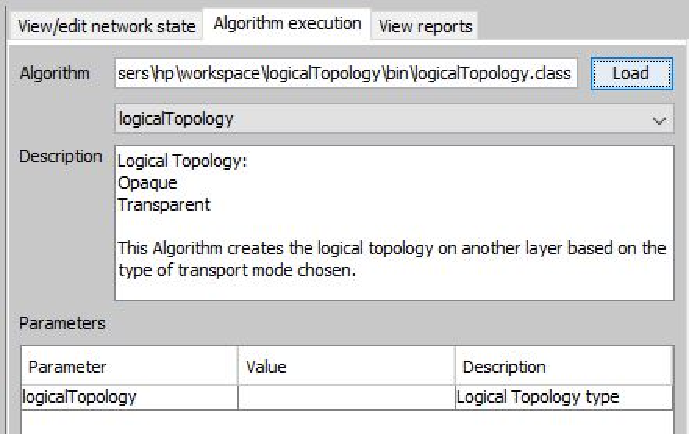
\includegraphics[width = 10.5cm]{Net2Plan_introduce_algorithm.pdf}
		\caption{Net2Plan new algorithm}
		\label{Net2Plan_introduce_algorithm}
	\end{figure}
			
				
			
	As was said before and can be seen on the "Description", this algorithm creates the network logical topology as was explained on section \ref{Creating the Network topologies}.
			
	Algorithms developed on Eclipse can be exported into a .jar file so on Net2Plan this file can be loaded and all the algorithms developed are shown in a list in the same manner as the ones that came with the Net2Plan installation. The export option can be accessed by going into File $\rightarrow$ Export, and the menu are shown in Figures \ref{Eclipse_export} and \ref{Eclipse_export_1}.
	
	\begin{figure}[!h]
		\centering
		\subfigure[]
		{
			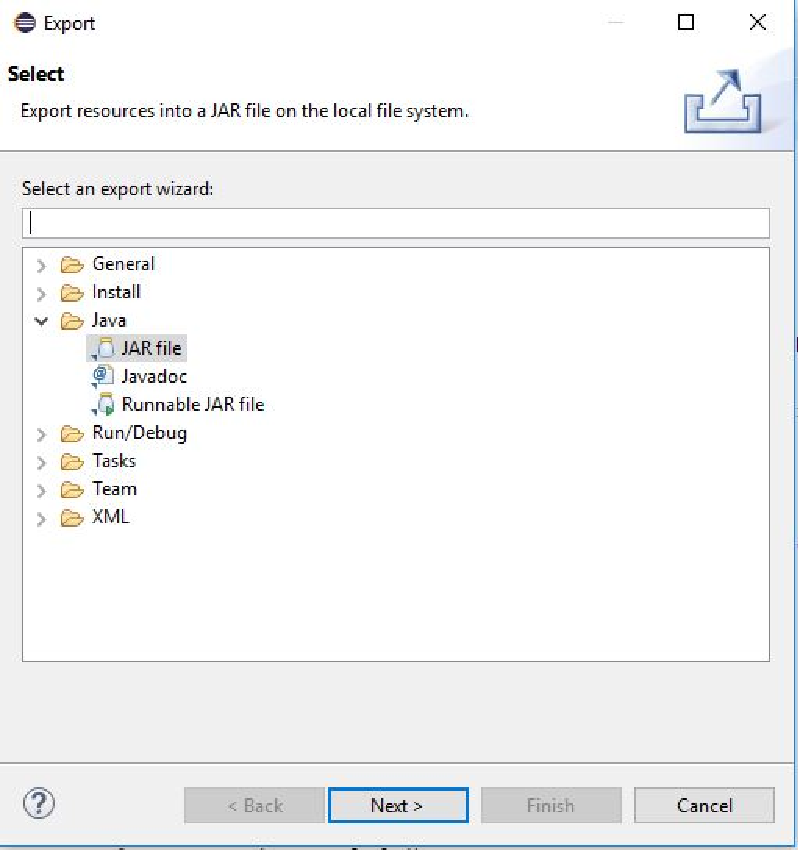
\includegraphics[width = 6cm]{Eclipse_export.pdf}
			\label{Eclipse_export}
		}
		\subfigure[]
		{
			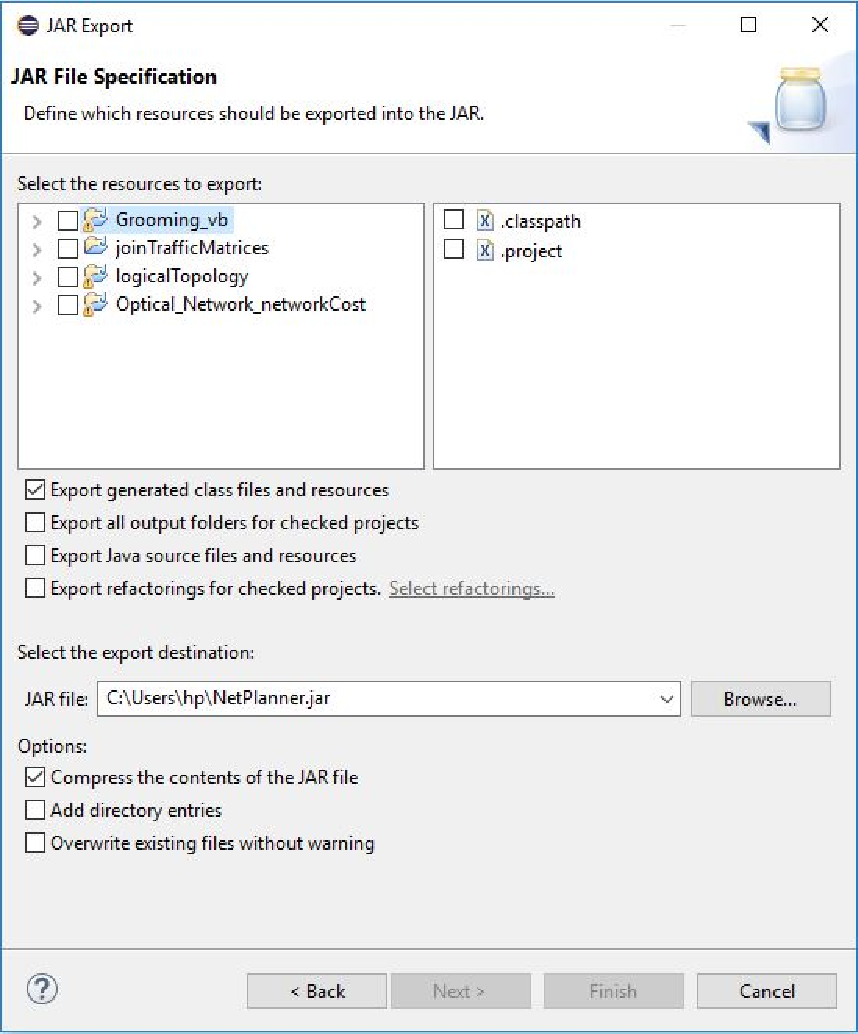
\includegraphics[width = 6cm]{Eclipse_export_1.pdf}
			\label{Eclipse_export_1}
		}
		\caption{a) Eclipse export ; b) Projects to export into a .jar file}
	\end{figure}
	
	By default only the .class files are exported along with the necessary libraries so that the algorithms can be loaded on Net2Plan. There is however an option to also export the .java files so that if needed the ones who will use the code also have access to it if they need to change it.
	 						
	\newpage

	\section*{Developing new Reports}
	Similarly to the way algorithms can be modified or new ones created, also reports can be done using almost the same steps. For the following examples, the "Optical\_Network\_networkcost" is being used as a basis for modifying or creating new reports.

	An important point to note as the main difference as to when modifying algorithms, is that in this case not only are the Net2Plan libraries needed but also the extra files summoned by the report. These files can be found opening the "BuiltInExamples.jar" file in the Net2Plan directory on the corresponding report.

	For the report being used there is an .html file called "main" which is where the information to be displayed in html form is described as well as several image files that are displayed in the report. As such, if the modifications to be done in the reports are to be shown in html format the "main.html" file needs to be modified in order to adapt to these changes.
	
	The tables themselves are created in eclipse as Java code but the html file needs to be opened for example with "Notepadd++" to change some its code as the tables are being appended into the html. Figure \ref{html_report} shows the modified html that is used in the Optical\_Network\_networkcost.
	
	\begin{figure}[h!]
		\centering
		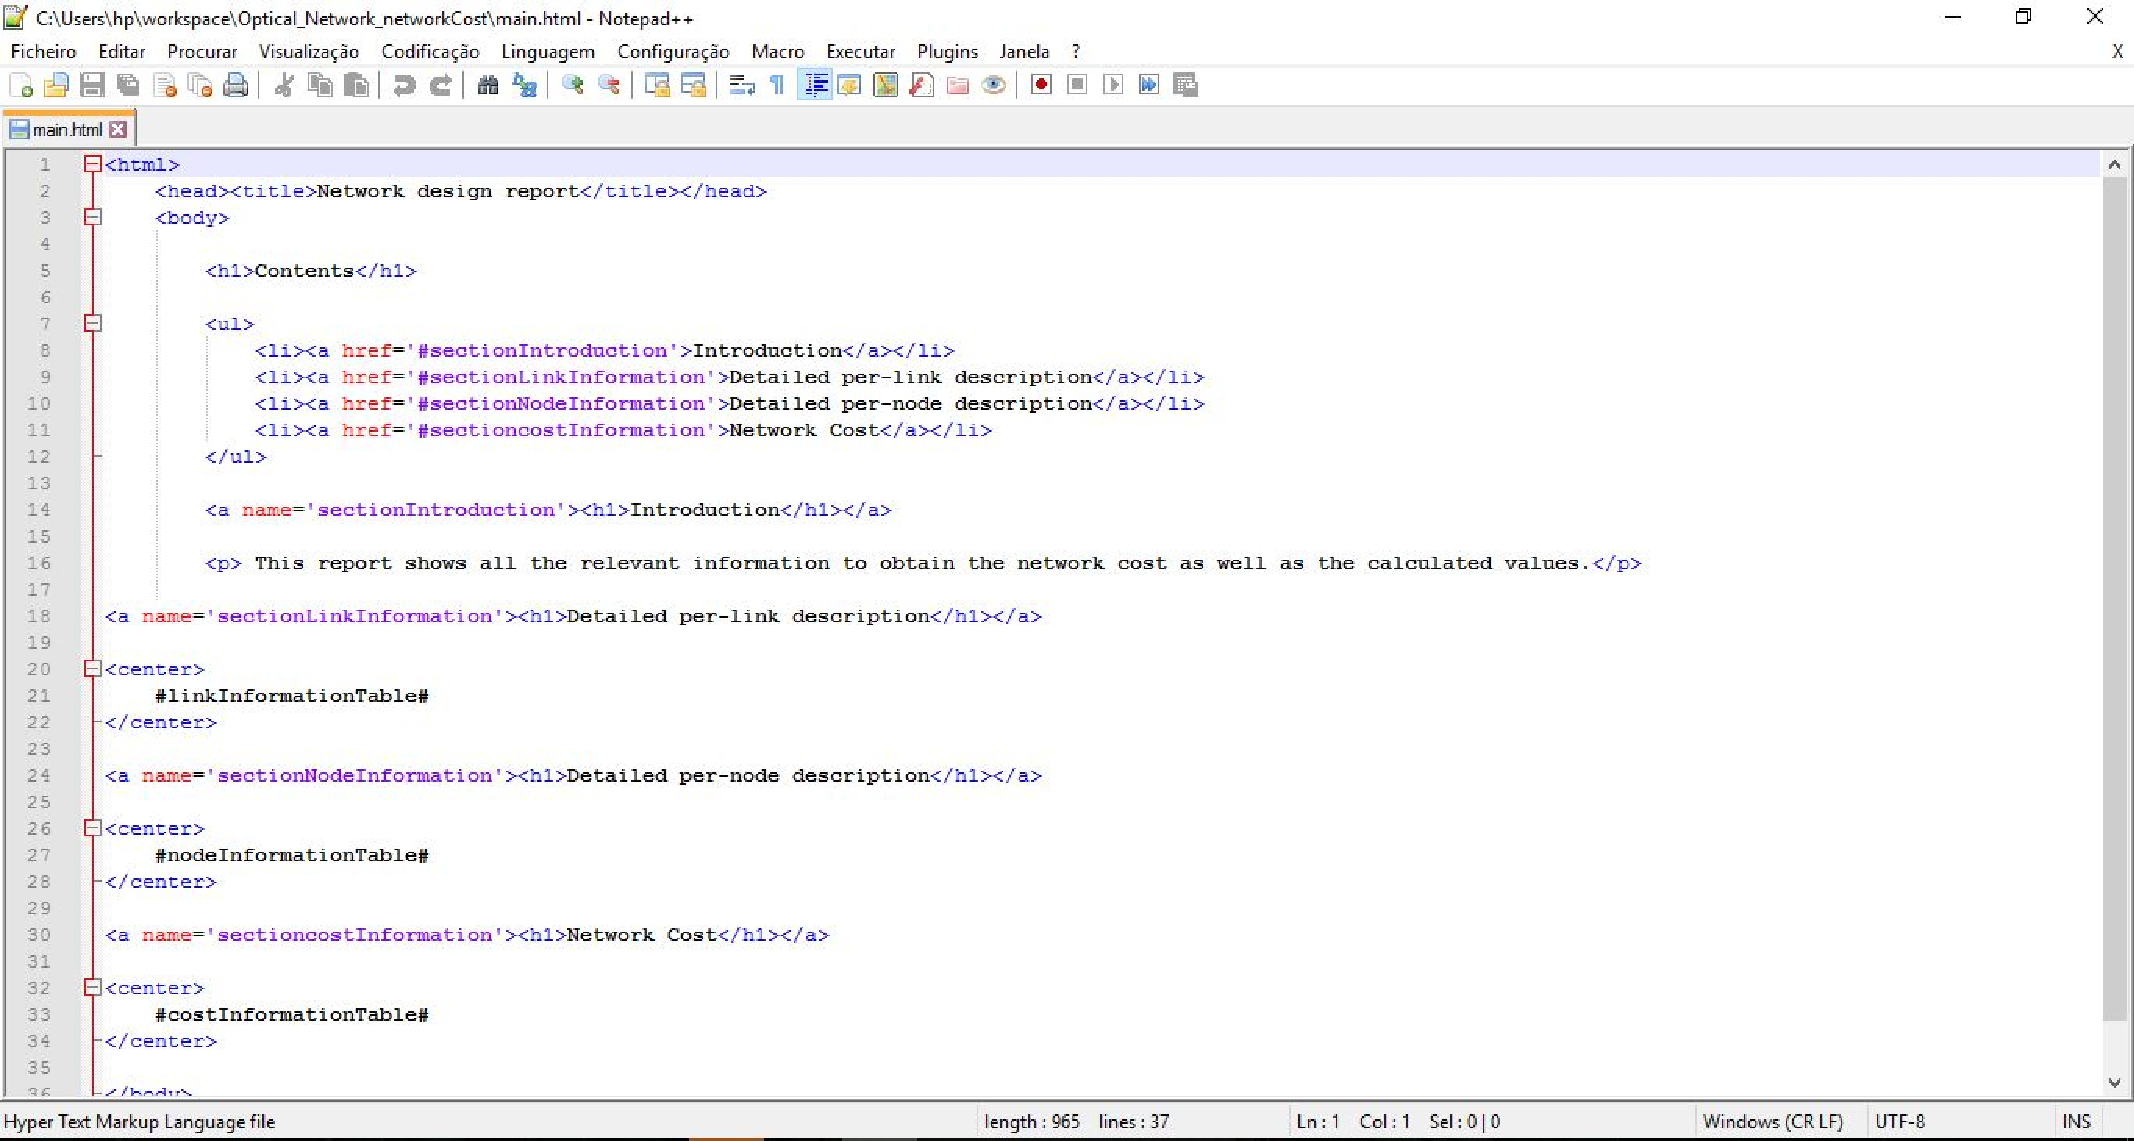
\includegraphics[width = 17cm]{html_report.pdf}
		\caption{html file for Network Cost report}
		\label{html_report}
	\end{figure}	
		
	As can be seen, this is a simple example of an html file since there are only hyper links created to link the contents index to the tables. Other options could be added as for example, hyper links to each of the network costs with the formula describing its calculations by adding the necessary information in this file. These extra options are present on more complex reports such as the "Report\_networkDesign" where the images used are equations showcasing how some of the calculations are done.
	
\clearpage

\subsubsection{Creation of traffic matrices}\label{creation_traffic_matrices}

Accordingly to the reference network in \label{Reference_Network_Traffic} and to the ODUs defined in \label{low_traffic_scenario} for the low, medium and high traffic scenario, we can create the traffic matrices with a constant traffic pattern. As all the network components are bidirectional, the amount of traffic that passes to all node pairs must be the same.

The next step is to choose the number of nodes, number of matrices and the constant value. For the network of reference it is used 6 nodes, 5 matrices and the constant has value 0. After inserted the values in each ODU matrix it is possible to save them and create now a network topological design.

\begin{figure}[h!]
\centering
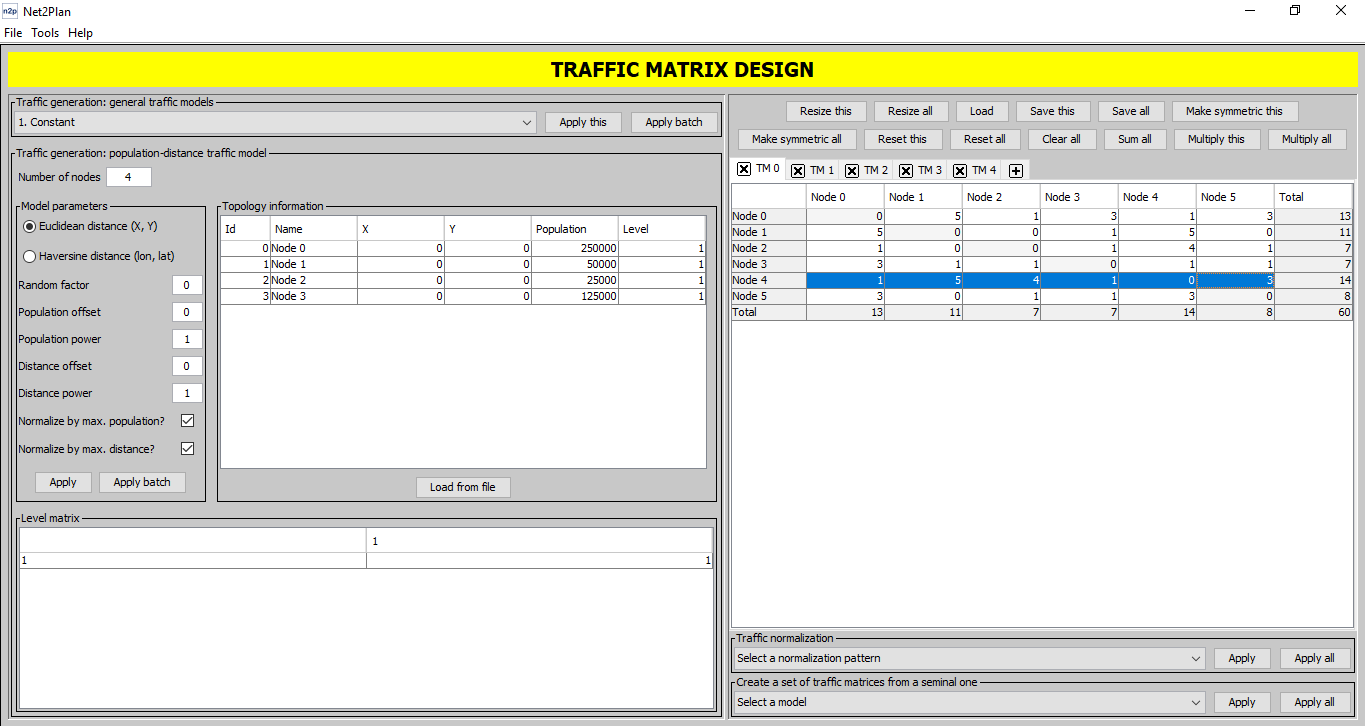
\includegraphics[width=12cm]{sdf/heuristic/figures/traffic_matrix_design}
\caption{Traffic matrix design using Net2Plan.}
\label{traffic_matrix_design}
\end{figure}

\subsubsection{Creation of a network topological design}\label{creation_topological_design}

\vspace{11pt}
To create the network topological design that was defined before in \label{creation_traffic_matrices} it is needed to add the 6 nodes that were chosen and link them with bidirectional links as it is shown in the picture \label{network_topological_design} below.

It is known that each node represents an end-node which has a certain number of transmitters and receivers for a communication. These nodes are connected by optical fibers that support a fixed number of wavelengths.

On the right side of the network design it is shown all the attributes of the network. However, some arguments are not set yet, like the capacity and the traffic demands that passes in each link, so now it is necessary to use routing and grooming algorithms in order to simulate the heuristic algorithms in this reference network.

\begin{figure}[h!]
\centering
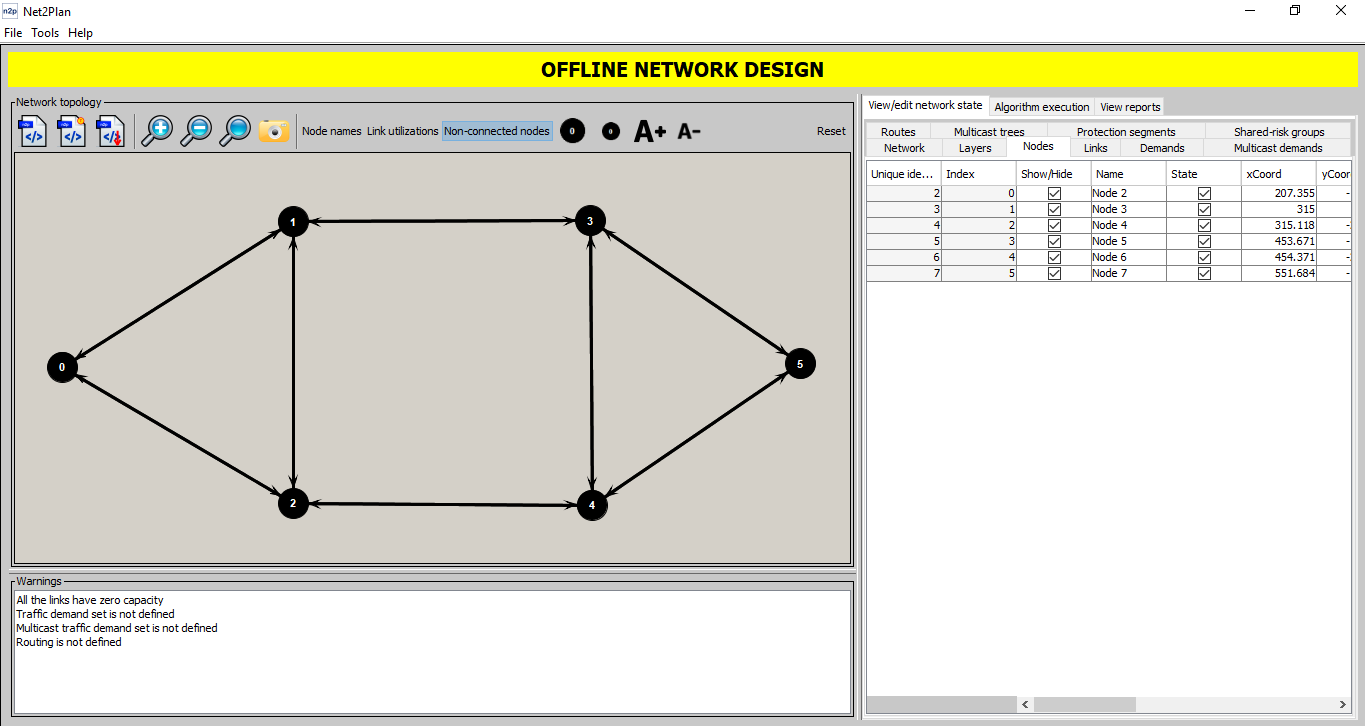
\includegraphics[width=12cm]{sdf/heuristic/figures/network_topological_design}
\caption{Network topological design using Net2Plan.}
\label{network_topological_design}
\end{figure}

\subsubsection{Join Traffic Matrices Algorithm}\label{join_traffic_matrices_algorithm}

\vspace{11pt}
The first algorithm used is the "Join Traffic Matrices" algorithm and it joins the traffic demands of the ODU traffic matrices into a file. This file will be used later for loading the traffic demands to the network topological design on Net2Plan. This algorithm aggregates the traffic matrices from ODU0 to ODU4. If it is used a network with multiple matrices and, respectively, multiple traffic demands it is possible to join each of them and save it.

\clearpage
\begin{figure}[h!]
\centering
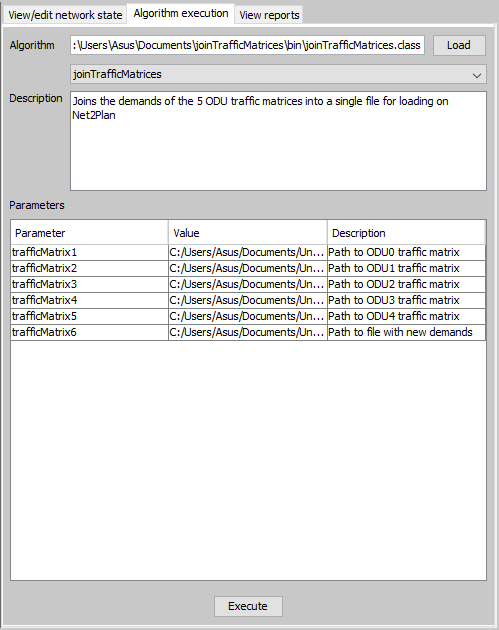
\includegraphics[width=10cm]{sdf/heuristic/figures/join_traffic_matrices}
\caption{Join traffic matrices algorithm using Net2Plan.}
\label{join_traffic_matrices}
\end{figure}

\subsubsection{Logical Topology Algorithm}\label{logical_topology_algorithm}

\vspace{11pt}
The "Logical Topology" algorithm is the second one used and it is based on the transport mode that is used in the network and it creates the logical topology on another layer. The logical topology value is introduced by the user and it can be one of the three transport modes available. If the transport mode chosen is opaque there is no need of having a second layer because the logical layer is the same as the physical one and if the transport mode is transparent or translucent it is needed to add a new logical layer. One advantage of this algorithm is that all the traffic demands are copied to the new layer and all the arguments remains the same depending on the previous layer, not interfering with the network topology.

It is also needed to add by the user the capacity that is used in each wavelength from all origin nodes to all destination nodes and the length of the links with values of the distance matrix represented in \label{Reference_Network_Topology} and expressed in km.

\begin{figure}[h!]
\centering
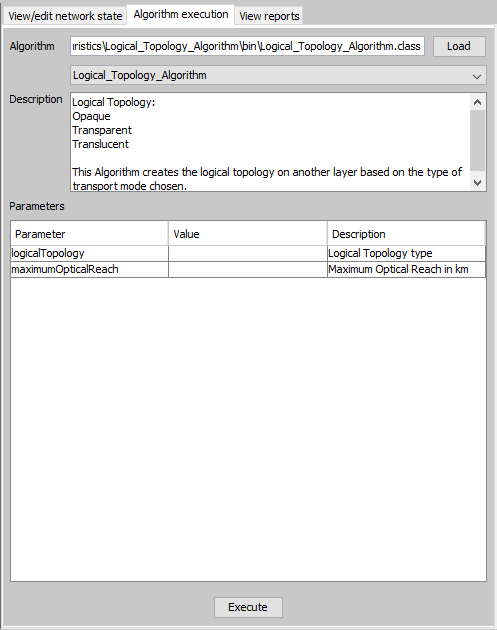
\includegraphics[width=10cm]{sdf/heuristic/figures/logical_topology}
\caption{Logical topology algorithm using Net2Plan.}
\label{logical_topology}
\end{figure}

\subsubsection{Grooming Algorithm}\label{grooming_algorithm}

\vspace{11pt}
The "Grooming" algorithm is a shortest-path heuristic algorithm that creates routes and protection paths based on hops or km, accordingly to the pre-defined logical topology. The goal of this grooming algorithm is to minimize the number of links for each path between all node pairs and this will lead to the reduction of the number of wavelengths to serve a set of connections and, consequently, to a lower cost of nodes and lower CAPEX.

The approach of the routing algorithm is to route all the traffic demands using the "Dijkstra" algorithm and uses the shortest number of hops to reach the destination node. The shortest path between two nodes is the one that includes connections whose sum of weights is the least possible. Routing through the shortest path consists in routing sequentially each element of a traffic matrix to the shortest path in the network. The routing is done in the logical and physical topologies of the network. In addition, the route from node o to d should be the opposite direction of node d to o as there could be different routes with the shortest path that are not using the same path. It is assumed that links are bidirectional and the traffic demands are given between pairs of nodes and a network topology. In this case, each wavelength will be served by two wavelength paths. If the number of used wavelengths is minimum, the number of used fibers will be also minimum, which minimizes the CAPEX.

The 1+1 protection scheme (dedicated path protection) assumes that each link has a dedicated protection communication channel. For this scenario, it is necessary to assign different wavelengths to the primary and protection paths. It is chosen the best path based on the shortest or disjointed path, for without survivability or with 1+1 protection, respectively. The optimization objective is to minimize the number of assigned wavelengths and network components.

\begin{figure}[h!]
\centering
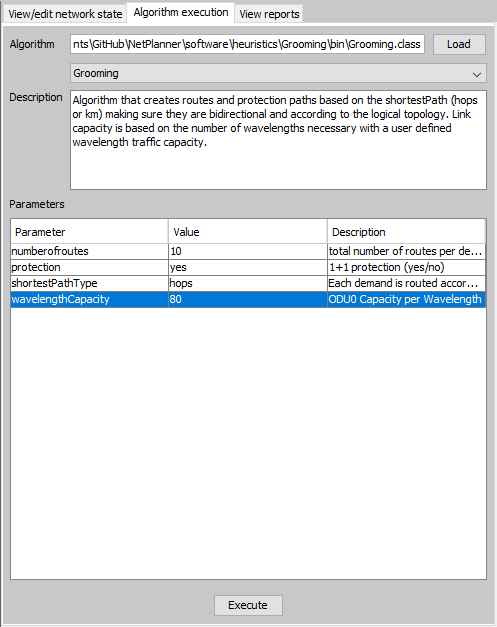
\includegraphics[width=10cm]{sdf/heuristic/figures/grooming}
\caption{Grooming algorithm using Net2Plan.}
\label{grooming}
\end{figure}
